\documentclass[twoside]{book}

% Packages required by doxygen
\usepackage{fixltx2e}
\usepackage{calc}
\usepackage{doxygen}
\usepackage[export]{adjustbox} % also loads graphicx
\usepackage{graphicx}
\usepackage[utf8]{inputenc}
\usepackage{makeidx}
\usepackage{multicol}
\usepackage{multirow}
\PassOptionsToPackage{warn}{textcomp}
\usepackage{textcomp}
\usepackage[nointegrals]{wasysym}
\usepackage[table]{xcolor}

% Font selection
\usepackage[T1]{fontenc}
\usepackage[scaled=.90]{helvet}
\usepackage{courier}
\usepackage{amssymb}
\usepackage{sectsty}
\renewcommand{\familydefault}{\sfdefault}
\allsectionsfont{%
  \fontseries{bc}\selectfont%
  \color{darkgray}%
}
\renewcommand{\DoxyLabelFont}{%
  \fontseries{bc}\selectfont%
  \color{darkgray}%
}
\newcommand{\+}{\discretionary{\mbox{\scriptsize$\hookleftarrow$}}{}{}}

% Page & text layout
\usepackage{geometry}
\geometry{%
  a4paper,%
  top=2.5cm,%
  bottom=2.5cm,%
  left=2.5cm,%
  right=2.5cm%
}
\tolerance=750
\hfuzz=15pt
\hbadness=750
\setlength{\emergencystretch}{15pt}
\setlength{\parindent}{0cm}
\setlength{\parskip}{3ex plus 2ex minus 2ex}
\makeatletter
\renewcommand{\paragraph}{%
  \@startsection{paragraph}{4}{0ex}{-1.0ex}{1.0ex}{%
    \normalfont\normalsize\bfseries\SS@parafont%
  }%
}
\renewcommand{\subparagraph}{%
  \@startsection{subparagraph}{5}{0ex}{-1.0ex}{1.0ex}{%
    \normalfont\normalsize\bfseries\SS@subparafont%
  }%
}
\makeatother

% Headers & footers
\usepackage{fancyhdr}
\pagestyle{fancyplain}
\fancyhead[LE]{\fancyplain{}{\bfseries\thepage}}
\fancyhead[CE]{\fancyplain{}{}}
\fancyhead[RE]{\fancyplain{}{\bfseries\leftmark}}
\fancyhead[LO]{\fancyplain{}{\bfseries\rightmark}}
\fancyhead[CO]{\fancyplain{}{}}
\fancyhead[RO]{\fancyplain{}{\bfseries\thepage}}
\fancyfoot[LE]{\fancyplain{}{}}
\fancyfoot[CE]{\fancyplain{}{}}
\fancyfoot[RE]{\fancyplain{}{\bfseries\scriptsize Generated by Doxygen }}
\fancyfoot[LO]{\fancyplain{}{\bfseries\scriptsize Generated by Doxygen }}
\fancyfoot[CO]{\fancyplain{}{}}
\fancyfoot[RO]{\fancyplain{}{}}
\renewcommand{\footrulewidth}{0.4pt}
\renewcommand{\chaptermark}[1]{%
  \markboth{#1}{}%
}
\renewcommand{\sectionmark}[1]{%
  \markright{\thesection\ #1}%
}

% Indices & bibliography
\usepackage{natbib}
\usepackage[titles]{tocloft}
\setcounter{tocdepth}{3}
\setcounter{secnumdepth}{5}
\makeindex

% Hyperlinks (required, but should be loaded last)
\usepackage{ifpdf}
\ifpdf
  \usepackage[pdftex,pagebackref=true]{hyperref}
\else
  \usepackage[ps2pdf,pagebackref=true]{hyperref}
\fi
\hypersetup{%
  colorlinks=true,%
  linkcolor=blue,%
  citecolor=blue,%
  unicode%
}

% Custom commands
\newcommand{\clearemptydoublepage}{%
  \newpage{\pagestyle{empty}\cleardoublepage}%
}

\usepackage{caption}
\captionsetup{labelsep=space,justification=centering,font={bf},singlelinecheck=off,skip=4pt,position=top}

%===== C O N T E N T S =====

\begin{document}

% Titlepage & ToC
\hypersetup{pageanchor=false,
             bookmarksnumbered=true,
             pdfencoding=unicode
            }
\pagenumbering{alph}
\begin{titlepage}
\vspace*{7cm}
\begin{center}%
{\Large My Project }\\
\vspace*{1cm}
{\large Generated by Doxygen 1.8.13}\\
\end{center}
\end{titlepage}
\clearemptydoublepage
\pagenumbering{roman}
\tableofcontents
\clearemptydoublepage
\pagenumbering{arabic}
\hypersetup{pageanchor=true}

%--- Begin generated contents ---
\chapter{Hierarchical Index}
\section{Class Hierarchy}
This inheritance list is sorted roughly, but not completely, alphabetically\+:\begin{DoxyCompactList}
\item \contentsline{section}{Cell\+Type}{\pageref{class_cell_type}}{}
\begin{DoxyCompactList}
\item \contentsline{section}{Cell\+Double}{\pageref{class_cell_double}}{}
\item \contentsline{section}{Cell\+Formula}{\pageref{class_cell_formula}}{}
\item \contentsline{section}{Cell\+Int}{\pageref{class_cell_int}}{}
\item \contentsline{section}{Cell\+String}{\pageref{class_cell_string}}{}
\end{DoxyCompactList}
\item \contentsline{section}{Command}{\pageref{class_command}}{}
\item \contentsline{section}{Spreadsheet}{\pageref{class_spreadsheet}}{}
\item \contentsline{section}{String}{\pageref{class_string}}{}
\item \contentsline{section}{Vector$<$ T $>$}{\pageref{class_vector}}{}
\end{DoxyCompactList}

\chapter{Class Index}
\section{Class List}
Here are the classes, structs, unions and interfaces with brief descriptions\+:\begin{DoxyCompactList}
\item\contentsline{section}{\hyperlink{class_cell_double}{Cell\+Double} \\*Class \hyperlink{class_cell_double}{Cell\+Double} description }{\pageref{class_cell_double}}{}
\item\contentsline{section}{\hyperlink{class_cell_formula}{Cell\+Formula} \\*Class \hyperlink{class_cell_formula}{Cell\+Formula} description }{\pageref{class_cell_formula}}{}
\item\contentsline{section}{\hyperlink{class_cell_int}{Cell\+Int} \\*Class \hyperlink{class_cell_int}{Cell\+Int} description }{\pageref{class_cell_int}}{}
\item\contentsline{section}{\hyperlink{class_cell_string}{Cell\+String} \\*Class \hyperlink{class_cell_string}{Cell\+String} description }{\pageref{class_cell_string}}{}
\item\contentsline{section}{\hyperlink{class_cell_type}{Cell\+Type} \\*Class \hyperlink{class_cell_type}{Cell\+Type} description }{\pageref{class_cell_type}}{}
\item\contentsline{section}{\hyperlink{class_command}{Command} \\*Class \hyperlink{class_command}{Command} description }{\pageref{class_command}}{}
\item\contentsline{section}{\hyperlink{class_spreadsheet}{Spreadsheet} \\*Class \hyperlink{class_spreadsheet}{Spreadsheet} description }{\pageref{class_spreadsheet}}{}
\item\contentsline{section}{\hyperlink{class_string}{String} \\*Class \hyperlink{class_string}{String} description }{\pageref{class_string}}{}
\item\contentsline{section}{\hyperlink{class_vector}{Vector$<$ T $>$} \\*Class \hyperlink{class_vector}{Vector} description }{\pageref{class_vector}}{}
\end{DoxyCompactList}

\chapter{Class Documentation}
\hypertarget{class_cell_double}{}\section{Cell\+Double Class Reference}
\label{class_cell_double}\index{Cell\+Double@{Cell\+Double}}


Class \hyperlink{class_cell_double}{Cell\+Double} description.  




{\ttfamily \#include $<$Cell\+Double.\+h$>$}

Inheritance diagram for Cell\+Double\+:\begin{figure}[H]
\begin{center}
\leavevmode
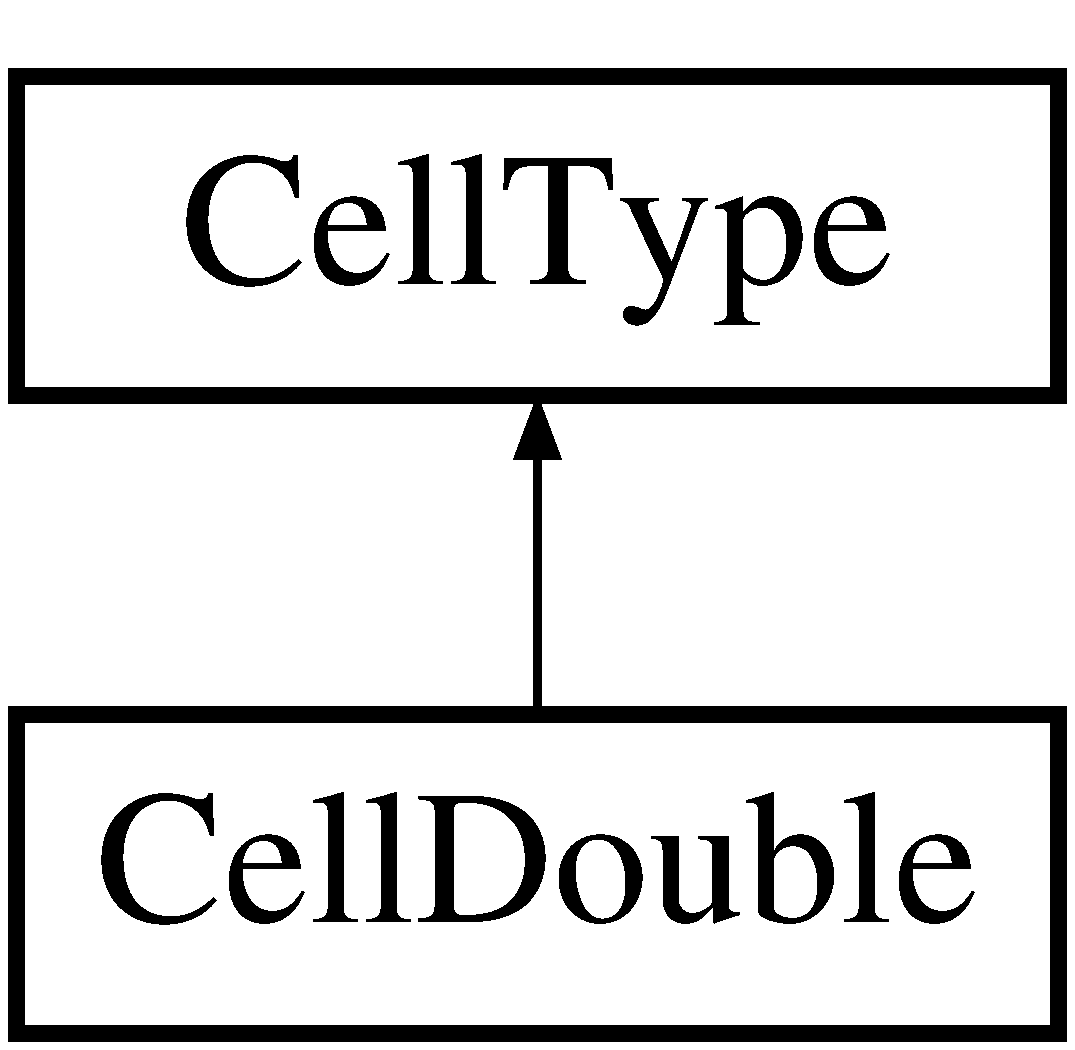
\includegraphics[height=2.000000cm]{class_cell_double}
\end{center}
\end{figure}
\subsection*{Public Member Functions}
\begin{DoxyCompactItemize}
\item 
\mbox{\Hypertarget{class_cell_double_a6ae1b712877cd64720282a51acc51d76}\label{class_cell_double_a6ae1b712877cd64720282a51acc51d76}} 
\hyperlink{class_cell_double_a6ae1b712877cd64720282a51acc51d76}{Cell\+Double} ()
\begin{DoxyCompactList}\small\item\em Default constructor. \end{DoxyCompactList}\item 
\mbox{\Hypertarget{class_cell_double_a0f4a236493a840fa3fe89a4ae2dbe1c1}\label{class_cell_double_a0f4a236493a840fa3fe89a4ae2dbe1c1}} 
\hyperlink{class_cell_double_a0f4a236493a840fa3fe89a4ae2dbe1c1}{Cell\+Double} (double number, \hyperlink{class_string}{String} String\+Number)
\begin{DoxyCompactList}\small\item\em Create new obj from assign value. \end{DoxyCompactList}\item 
virtual \hyperlink{class_cell_type}{Cell\+Type} $\ast$ \hyperlink{class_cell_double_a8d378687ae89338267e61d61ff932680}{clone} () const
\item 
virtual void \hyperlink{class_cell_double_a90539ceb6daa29e7b658d8f2a2d1445d}{print} (std\+::ostream \&out) const
\item 
virtual unsigned \hyperlink{class_cell_double_ac2d36517f1107fb0271172ea30d6bff5}{lenght} () const
\item 
virtual double \hyperlink{class_cell_double_a6ed39c7b32c0599b4db0f046c7cfab93}{value} () const
\item 
virtual \hyperlink{class_string}{String} \hyperlink{class_cell_double_a73662d15e8626c81858e3a243f0d6818}{type} () const
\item 
virtual \hyperlink{class_string}{String} \hyperlink{class_cell_double_a3e92f9ec4b564b3e14fa829529bbaf0a}{string\+Cell} () const
\end{DoxyCompactItemize}


\subsection{Detailed Description}
Class \hyperlink{class_cell_double}{Cell\+Double} description. 

double type of the cell derivated class at \hyperlink{class_cell_type}{Cell\+Type} 

\subsection{Member Function Documentation}
\mbox{\Hypertarget{class_cell_double_a8d378687ae89338267e61d61ff932680}\label{class_cell_double_a8d378687ae89338267e61d61ff932680}} 
\index{Cell\+Double@{Cell\+Double}!clone@{clone}}
\index{clone@{clone}!Cell\+Double@{Cell\+Double}}
\subsubsection{\texorpdfstring{clone()}{clone()}}
{\footnotesize\ttfamily \hyperlink{class_cell_type}{Cell\+Type} $\ast$ Cell\+Double\+::clone (\begin{DoxyParamCaption}{ }\end{DoxyParamCaption}) const\hspace{0.3cm}{\ttfamily [virtual]}}

Derivate class can be cloned -\/ Returns pointer to himself 

Implements \hyperlink{class_cell_type_a8c534b1eed27659429f761fc76d51b89}{Cell\+Type}.

\mbox{\Hypertarget{class_cell_double_ac2d36517f1107fb0271172ea30d6bff5}\label{class_cell_double_ac2d36517f1107fb0271172ea30d6bff5}} 
\index{Cell\+Double@{Cell\+Double}!lenght@{lenght}}
\index{lenght@{lenght}!Cell\+Double@{Cell\+Double}}
\subsubsection{\texorpdfstring{lenght()}{lenght()}}
{\footnotesize\ttfamily unsigned Cell\+Double\+::lenght (\begin{DoxyParamCaption}{ }\end{DoxyParamCaption}) const\hspace{0.3cm}{\ttfamily [virtual]}}

Return lenght of the Cell type 

Implements \hyperlink{class_cell_type_a1f8bd268dbd474dd8e08726a6efac066}{Cell\+Type}.

\mbox{\Hypertarget{class_cell_double_a90539ceb6daa29e7b658d8f2a2d1445d}\label{class_cell_double_a90539ceb6daa29e7b658d8f2a2d1445d}} 
\index{Cell\+Double@{Cell\+Double}!print@{print}}
\index{print@{print}!Cell\+Double@{Cell\+Double}}
\subsubsection{\texorpdfstring{print()}{print()}}
{\footnotesize\ttfamily void Cell\+Double\+::print (\begin{DoxyParamCaption}\item[{std\+::ostream \&}]{out }\end{DoxyParamCaption}) const\hspace{0.3cm}{\ttfamily [virtual]}}

Print on the stream given as the first argument 

Implements \hyperlink{class_cell_type_a34413fcb76f292b6b8d08615765ba894}{Cell\+Type}.

\mbox{\Hypertarget{class_cell_double_a3e92f9ec4b564b3e14fa829529bbaf0a}\label{class_cell_double_a3e92f9ec4b564b3e14fa829529bbaf0a}} 
\index{Cell\+Double@{Cell\+Double}!string\+Cell@{string\+Cell}}
\index{string\+Cell@{string\+Cell}!Cell\+Double@{Cell\+Double}}
\subsubsection{\texorpdfstring{string\+Cell()}{stringCell()}}
{\footnotesize\ttfamily \hyperlink{class_string}{String} Cell\+Double\+::string\+Cell (\begin{DoxyParamCaption}{ }\end{DoxyParamCaption}) const\hspace{0.3cm}{\ttfamily [virtual]}}

Return a content of the cell 

Implements \hyperlink{class_cell_type_abba4d6d43efa340144d1ad09637e1aa9}{Cell\+Type}.

\mbox{\Hypertarget{class_cell_double_a73662d15e8626c81858e3a243f0d6818}\label{class_cell_double_a73662d15e8626c81858e3a243f0d6818}} 
\index{Cell\+Double@{Cell\+Double}!type@{type}}
\index{type@{type}!Cell\+Double@{Cell\+Double}}
\subsubsection{\texorpdfstring{type()}{type()}}
{\footnotesize\ttfamily \hyperlink{class_string}{String} Cell\+Double\+::type (\begin{DoxyParamCaption}{ }\end{DoxyParamCaption}) const\hspace{0.3cm}{\ttfamily [virtual]}}

Return Cell type name 

Implements \hyperlink{class_cell_type_ae31acfe1efc7776796d85918886247af}{Cell\+Type}.

\mbox{\Hypertarget{class_cell_double_a6ed39c7b32c0599b4db0f046c7cfab93}\label{class_cell_double_a6ed39c7b32c0599b4db0f046c7cfab93}} 
\index{Cell\+Double@{Cell\+Double}!value@{value}}
\index{value@{value}!Cell\+Double@{Cell\+Double}}
\subsubsection{\texorpdfstring{value()}{value()}}
{\footnotesize\ttfamily double Cell\+Double\+::value (\begin{DoxyParamCaption}{ }\end{DoxyParamCaption}) const\hspace{0.3cm}{\ttfamily [virtual]}}

Return value of the Cell type 

Implements \hyperlink{class_cell_type_a6cbfc477f605049f2a007d8674442230}{Cell\+Type}.



The documentation for this class was generated from the following files\+:\begin{DoxyCompactItemize}
\item 
D\+:/ФМИ/\+I\+I semestyr/\+O\+O\+P/fn45311 Spreadsheet project-\/updated/\+Project Speadsheets/Cell\+Double.\+h\item 
D\+:/ФМИ/\+I\+I semestyr/\+O\+O\+P/fn45311 Spreadsheet project-\/updated/\+Project Speadsheets/Cell\+Double.\+cpp\end{DoxyCompactItemize}

\hypertarget{class_cell_formula}{}\section{Cell\+Formula Class Reference}
\label{class_cell_formula}\index{Cell\+Formula@{Cell\+Formula}}


Class \hyperlink{class_cell_formula}{Cell\+Formula} description.  




{\ttfamily \#include $<$Cell\+Formula.\+h$>$}

Inheritance diagram for Cell\+Formula\+:\begin{figure}[H]
\begin{center}
\leavevmode
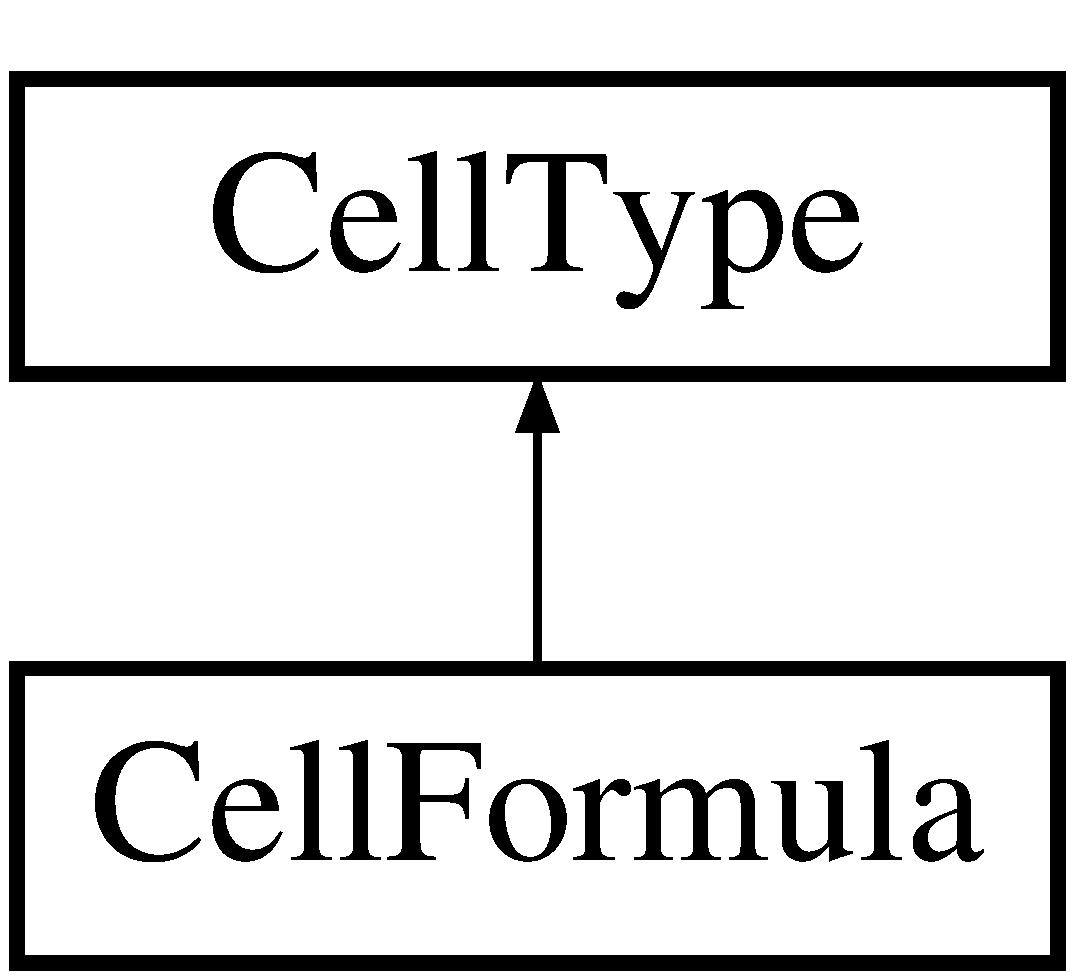
\includegraphics[height=2.000000cm]{class_cell_formula}
\end{center}
\end{figure}
\subsection*{Public Member Functions}
\begin{DoxyCompactItemize}
\item 
\mbox{\Hypertarget{class_cell_formula_a6cec93558e2c0a980fab7e82596ad525}\label{class_cell_formula_a6cec93558e2c0a980fab7e82596ad525}} 
\hyperlink{class_cell_formula_a6cec93558e2c0a980fab7e82596ad525}{Cell\+Formula} ()
\begin{DoxyCompactList}\small\item\em Default constructor. \end{DoxyCompactList}\item 
\mbox{\Hypertarget{class_cell_formula_a45c45a54409a55c582bd3014ed1ded3a}\label{class_cell_formula_a45c45a54409a55c582bd3014ed1ded3a}} 
\hyperlink{class_cell_formula_a45c45a54409a55c582bd3014ed1ded3a}{Cell\+Formula} (const \hyperlink{class_string}{String} rhs)
\begin{DoxyCompactList}\small\item\em Create new obj from \hyperlink{class_string}{String}. \end{DoxyCompactList}\item 
\mbox{\Hypertarget{class_cell_formula_a827017b1efe9ed2891a293cc80469559}\label{class_cell_formula_a827017b1efe9ed2891a293cc80469559}} 
\hyperlink{class_cell_formula_a827017b1efe9ed2891a293cc80469559}{Cell\+Formula} (const char $\ast$text)
\begin{DoxyCompactList}\small\item\em Create new obj from char array. \end{DoxyCompactList}\item 
virtual \hyperlink{class_cell_type}{Cell\+Type} $\ast$ \hyperlink{class_cell_formula_a23c26c40ef7056d9395ed8bc4ebef3b9}{clone} () const
\item 
virtual void \hyperlink{class_cell_formula_ac8cfeff2585811ee01acb7a4ddf25723}{print} (std\+::ostream \&out) const
\item 
virtual unsigned \hyperlink{class_cell_formula_af188e3f639245c126e0ae30e17b8d3c0}{lenght} () const
\item 
virtual double \hyperlink{class_cell_formula_a29d9e3000ae3f0b0ebac72807a455fec}{value} () const
\item 
virtual \hyperlink{class_string}{String} \hyperlink{class_cell_formula_ae175fd79ee036efa3a968f37b8eb53bc}{type} () const
\item 
virtual \hyperlink{class_string}{String} \hyperlink{class_cell_formula_abe70a7ace4b58fe4154bacccb5e3c12c}{string\+Cell} () const
\end{DoxyCompactItemize}


\subsection{Detailed Description}
Class \hyperlink{class_cell_formula}{Cell\+Formula} description. 

Formula cell type derivated class at \hyperlink{class_cell_type}{Cell\+Type} The formula will be validated and calculated in the Speadsheet 

\subsection{Member Function Documentation}
\mbox{\Hypertarget{class_cell_formula_a23c26c40ef7056d9395ed8bc4ebef3b9}\label{class_cell_formula_a23c26c40ef7056d9395ed8bc4ebef3b9}} 
\index{Cell\+Formula@{Cell\+Formula}!clone@{clone}}
\index{clone@{clone}!Cell\+Formula@{Cell\+Formula}}
\subsubsection{\texorpdfstring{clone()}{clone()}}
{\footnotesize\ttfamily \hyperlink{class_cell_type}{Cell\+Type} $\ast$ Cell\+Formula\+::clone (\begin{DoxyParamCaption}{ }\end{DoxyParamCaption}) const\hspace{0.3cm}{\ttfamily [virtual]}}

Derivate class can be cloned -\/ Returns pointer to himself 

Implements \hyperlink{class_cell_type_a8c534b1eed27659429f761fc76d51b89}{Cell\+Type}.

\mbox{\Hypertarget{class_cell_formula_af188e3f639245c126e0ae30e17b8d3c0}\label{class_cell_formula_af188e3f639245c126e0ae30e17b8d3c0}} 
\index{Cell\+Formula@{Cell\+Formula}!lenght@{lenght}}
\index{lenght@{lenght}!Cell\+Formula@{Cell\+Formula}}
\subsubsection{\texorpdfstring{lenght()}{lenght()}}
{\footnotesize\ttfamily unsigned Cell\+Formula\+::lenght (\begin{DoxyParamCaption}{ }\end{DoxyParamCaption}) const\hspace{0.3cm}{\ttfamily [virtual]}}

Return lenght of the Cell type 

Implements \hyperlink{class_cell_type_a1f8bd268dbd474dd8e08726a6efac066}{Cell\+Type}.

\mbox{\Hypertarget{class_cell_formula_ac8cfeff2585811ee01acb7a4ddf25723}\label{class_cell_formula_ac8cfeff2585811ee01acb7a4ddf25723}} 
\index{Cell\+Formula@{Cell\+Formula}!print@{print}}
\index{print@{print}!Cell\+Formula@{Cell\+Formula}}
\subsubsection{\texorpdfstring{print()}{print()}}
{\footnotesize\ttfamily void Cell\+Formula\+::print (\begin{DoxyParamCaption}\item[{std\+::ostream \&}]{out }\end{DoxyParamCaption}) const\hspace{0.3cm}{\ttfamily [virtual]}}

Print on the stream given as the first argument 

Implements \hyperlink{class_cell_type_a34413fcb76f292b6b8d08615765ba894}{Cell\+Type}.

\mbox{\Hypertarget{class_cell_formula_abe70a7ace4b58fe4154bacccb5e3c12c}\label{class_cell_formula_abe70a7ace4b58fe4154bacccb5e3c12c}} 
\index{Cell\+Formula@{Cell\+Formula}!string\+Cell@{string\+Cell}}
\index{string\+Cell@{string\+Cell}!Cell\+Formula@{Cell\+Formula}}
\subsubsection{\texorpdfstring{string\+Cell()}{stringCell()}}
{\footnotesize\ttfamily \hyperlink{class_string}{String} Cell\+Formula\+::string\+Cell (\begin{DoxyParamCaption}{ }\end{DoxyParamCaption}) const\hspace{0.3cm}{\ttfamily [virtual]}}

Return a content of the cell 

Implements \hyperlink{class_cell_type_abba4d6d43efa340144d1ad09637e1aa9}{Cell\+Type}.

\mbox{\Hypertarget{class_cell_formula_ae175fd79ee036efa3a968f37b8eb53bc}\label{class_cell_formula_ae175fd79ee036efa3a968f37b8eb53bc}} 
\index{Cell\+Formula@{Cell\+Formula}!type@{type}}
\index{type@{type}!Cell\+Formula@{Cell\+Formula}}
\subsubsection{\texorpdfstring{type()}{type()}}
{\footnotesize\ttfamily \hyperlink{class_string}{String} Cell\+Formula\+::type (\begin{DoxyParamCaption}{ }\end{DoxyParamCaption}) const\hspace{0.3cm}{\ttfamily [virtual]}}

Return Cell type name 

Implements \hyperlink{class_cell_type_ae31acfe1efc7776796d85918886247af}{Cell\+Type}.

\mbox{\Hypertarget{class_cell_formula_a29d9e3000ae3f0b0ebac72807a455fec}\label{class_cell_formula_a29d9e3000ae3f0b0ebac72807a455fec}} 
\index{Cell\+Formula@{Cell\+Formula}!value@{value}}
\index{value@{value}!Cell\+Formula@{Cell\+Formula}}
\subsubsection{\texorpdfstring{value()}{value()}}
{\footnotesize\ttfamily double Cell\+Formula\+::value (\begin{DoxyParamCaption}{ }\end{DoxyParamCaption}) const\hspace{0.3cm}{\ttfamily [virtual]}}

Return value of the Cell type 

Implements \hyperlink{class_cell_type_a6cbfc477f605049f2a007d8674442230}{Cell\+Type}.



The documentation for this class was generated from the following files\+:\begin{DoxyCompactItemize}
\item 
D\+:/ФМИ/\+I\+I semestyr/\+O\+O\+P/fn45311 Spreadsheet project-\/updated/\+Project Speadsheets/Cell\+Formula.\+h\item 
D\+:/ФМИ/\+I\+I semestyr/\+O\+O\+P/fn45311 Spreadsheet project-\/updated/\+Project Speadsheets/Cell\+Formula.\+cpp\end{DoxyCompactItemize}

\hypertarget{class_cell_int}{}\section{Cell\+Int Class Reference}
\label{class_cell_int}\index{Cell\+Int@{Cell\+Int}}


Class \hyperlink{class_cell_int}{Cell\+Int} description.  




{\ttfamily \#include $<$Cell\+Int.\+h$>$}

Inheritance diagram for Cell\+Int\+:\begin{figure}[H]
\begin{center}
\leavevmode
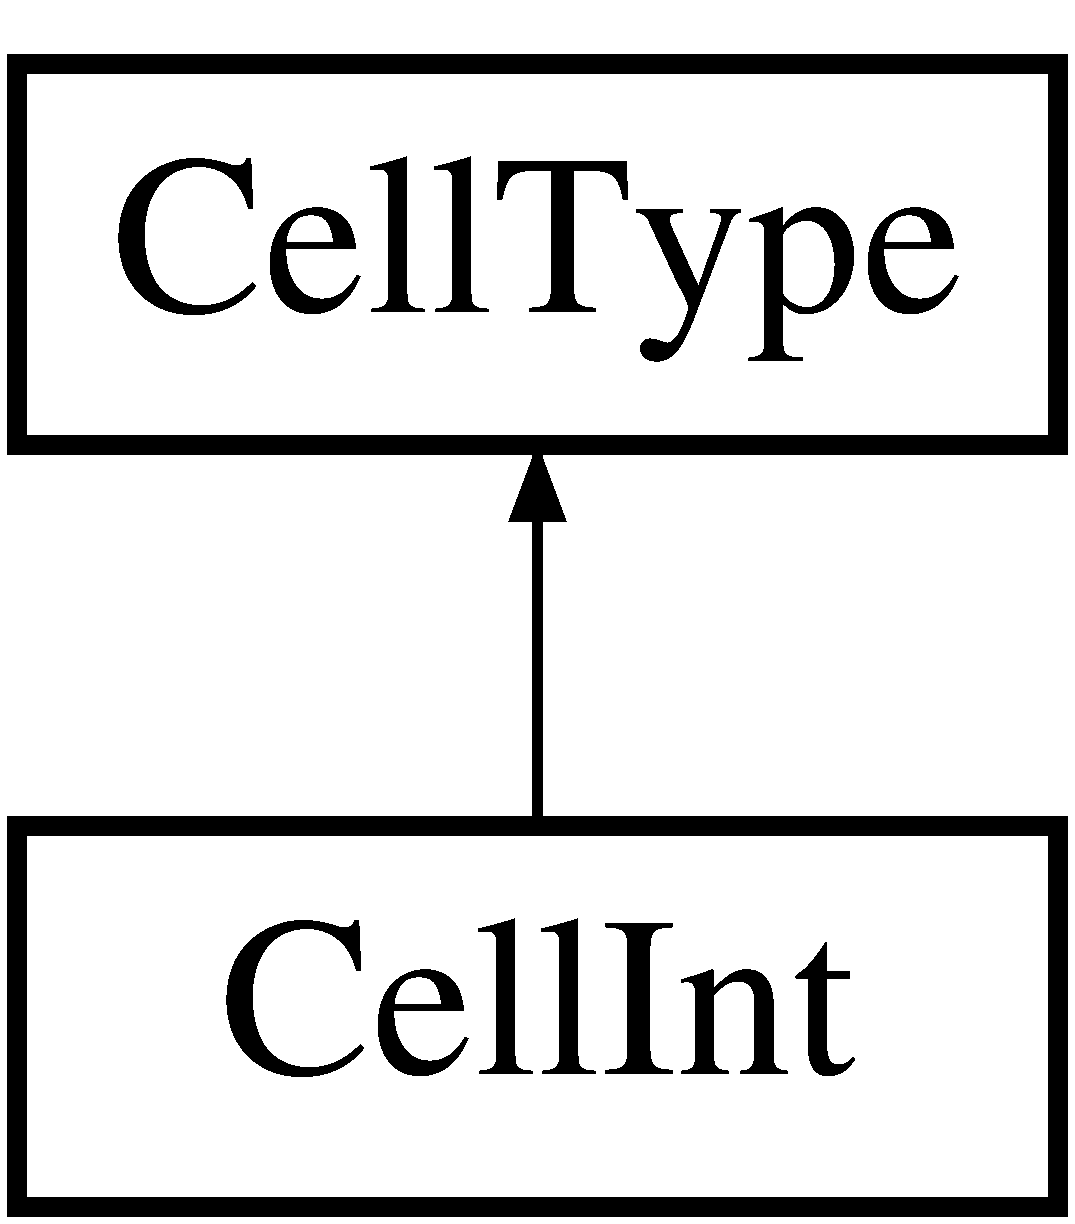
\includegraphics[height=2.000000cm]{class_cell_int}
\end{center}
\end{figure}
\subsection*{Public Member Functions}
\begin{DoxyCompactItemize}
\item 
\mbox{\Hypertarget{class_cell_int_a78dcfbea831221d91cb59dc730c33fe3}\label{class_cell_int_a78dcfbea831221d91cb59dc730c33fe3}} 
\hyperlink{class_cell_int_a78dcfbea831221d91cb59dc730c33fe3}{Cell\+Int} ()
\begin{DoxyCompactList}\small\item\em Default constructor. \end{DoxyCompactList}\item 
\mbox{\Hypertarget{class_cell_int_a103804b6b564d7fea54e84b369e0baff}\label{class_cell_int_a103804b6b564d7fea54e84b369e0baff}} 
\hyperlink{class_cell_int_a103804b6b564d7fea54e84b369e0baff}{Cell\+Int} (int number, \hyperlink{class_string}{String} String\+Number)
\begin{DoxyCompactList}\small\item\em Create new obj from assign value. \end{DoxyCompactList}\item 
virtual \hyperlink{class_cell_type}{Cell\+Type} $\ast$ \hyperlink{class_cell_int_a767b15d99c5ec0e2594dc35300e51873}{clone} () const
\item 
virtual void \hyperlink{class_cell_int_a1cb8461721999308790d105adff41cd2}{print} (std\+::ostream \&out) const
\item 
virtual unsigned \hyperlink{class_cell_int_afcab8270ff1853a08460051e02e62ace}{lenght} () const
\item 
virtual double \hyperlink{class_cell_int_a1be32d235fbcc58483948770fb7ce9c6}{value} () const
\item 
virtual \hyperlink{class_string}{String} \hyperlink{class_cell_int_a65c7fa9731cc6f5b40579f314ba090dd}{type} () const
\item 
virtual \hyperlink{class_string}{String} \hyperlink{class_cell_int_ae6b32857bc96f305fff4226c988032d4}{string\+Cell} () const
\end{DoxyCompactItemize}


\subsection{Detailed Description}
Class \hyperlink{class_cell_int}{Cell\+Int} description. 

int type of the cell derivated class at \hyperlink{class_cell_type}{Cell\+Type} 

\subsection{Member Function Documentation}
\mbox{\Hypertarget{class_cell_int_a767b15d99c5ec0e2594dc35300e51873}\label{class_cell_int_a767b15d99c5ec0e2594dc35300e51873}} 
\index{Cell\+Int@{Cell\+Int}!clone@{clone}}
\index{clone@{clone}!Cell\+Int@{Cell\+Int}}
\subsubsection{\texorpdfstring{clone()}{clone()}}
{\footnotesize\ttfamily \hyperlink{class_cell_type}{Cell\+Type} $\ast$ Cell\+Int\+::clone (\begin{DoxyParamCaption}{ }\end{DoxyParamCaption}) const\hspace{0.3cm}{\ttfamily [virtual]}}

Derivate class can be cloned -\/ Returns pointer to himself 

Implements \hyperlink{class_cell_type_a8c534b1eed27659429f761fc76d51b89}{Cell\+Type}.

\mbox{\Hypertarget{class_cell_int_afcab8270ff1853a08460051e02e62ace}\label{class_cell_int_afcab8270ff1853a08460051e02e62ace}} 
\index{Cell\+Int@{Cell\+Int}!lenght@{lenght}}
\index{lenght@{lenght}!Cell\+Int@{Cell\+Int}}
\subsubsection{\texorpdfstring{lenght()}{lenght()}}
{\footnotesize\ttfamily unsigned Cell\+Int\+::lenght (\begin{DoxyParamCaption}{ }\end{DoxyParamCaption}) const\hspace{0.3cm}{\ttfamily [virtual]}}

Return lenght of the Cell type 

Implements \hyperlink{class_cell_type_a1f8bd268dbd474dd8e08726a6efac066}{Cell\+Type}.

\mbox{\Hypertarget{class_cell_int_a1cb8461721999308790d105adff41cd2}\label{class_cell_int_a1cb8461721999308790d105adff41cd2}} 
\index{Cell\+Int@{Cell\+Int}!print@{print}}
\index{print@{print}!Cell\+Int@{Cell\+Int}}
\subsubsection{\texorpdfstring{print()}{print()}}
{\footnotesize\ttfamily void Cell\+Int\+::print (\begin{DoxyParamCaption}\item[{std\+::ostream \&}]{out }\end{DoxyParamCaption}) const\hspace{0.3cm}{\ttfamily [virtual]}}

Print on the stream given as the first argument 

Implements \hyperlink{class_cell_type_a34413fcb76f292b6b8d08615765ba894}{Cell\+Type}.

\mbox{\Hypertarget{class_cell_int_ae6b32857bc96f305fff4226c988032d4}\label{class_cell_int_ae6b32857bc96f305fff4226c988032d4}} 
\index{Cell\+Int@{Cell\+Int}!string\+Cell@{string\+Cell}}
\index{string\+Cell@{string\+Cell}!Cell\+Int@{Cell\+Int}}
\subsubsection{\texorpdfstring{string\+Cell()}{stringCell()}}
{\footnotesize\ttfamily \hyperlink{class_string}{String} Cell\+Int\+::string\+Cell (\begin{DoxyParamCaption}{ }\end{DoxyParamCaption}) const\hspace{0.3cm}{\ttfamily [virtual]}}

Return a content of the cell 

Implements \hyperlink{class_cell_type_abba4d6d43efa340144d1ad09637e1aa9}{Cell\+Type}.

\mbox{\Hypertarget{class_cell_int_a65c7fa9731cc6f5b40579f314ba090dd}\label{class_cell_int_a65c7fa9731cc6f5b40579f314ba090dd}} 
\index{Cell\+Int@{Cell\+Int}!type@{type}}
\index{type@{type}!Cell\+Int@{Cell\+Int}}
\subsubsection{\texorpdfstring{type()}{type()}}
{\footnotesize\ttfamily \hyperlink{class_string}{String} Cell\+Int\+::type (\begin{DoxyParamCaption}{ }\end{DoxyParamCaption}) const\hspace{0.3cm}{\ttfamily [virtual]}}

Return Cell type name 

Implements \hyperlink{class_cell_type_ae31acfe1efc7776796d85918886247af}{Cell\+Type}.

\mbox{\Hypertarget{class_cell_int_a1be32d235fbcc58483948770fb7ce9c6}\label{class_cell_int_a1be32d235fbcc58483948770fb7ce9c6}} 
\index{Cell\+Int@{Cell\+Int}!value@{value}}
\index{value@{value}!Cell\+Int@{Cell\+Int}}
\subsubsection{\texorpdfstring{value()}{value()}}
{\footnotesize\ttfamily double Cell\+Int\+::value (\begin{DoxyParamCaption}{ }\end{DoxyParamCaption}) const\hspace{0.3cm}{\ttfamily [virtual]}}

Return value of the Cell type 

Implements \hyperlink{class_cell_type_a6cbfc477f605049f2a007d8674442230}{Cell\+Type}.



The documentation for this class was generated from the following files\+:\begin{DoxyCompactItemize}
\item 
D\+:/ФМИ/\+I\+I semestyr/\+O\+O\+P/fn45311 Spreadsheet project-\/updated/\+Project Speadsheets/Cell\+Int.\+h\item 
D\+:/ФМИ/\+I\+I semestyr/\+O\+O\+P/fn45311 Spreadsheet project-\/updated/\+Project Speadsheets/Cell\+Int.\+cpp\end{DoxyCompactItemize}

\hypertarget{class_cell_string}{}\section{Cell\+String Class Reference}
\label{class_cell_string}\index{Cell\+String@{Cell\+String}}


Class \hyperlink{class_cell_string}{Cell\+String} description.  




{\ttfamily \#include $<$Cell\+String.\+h$>$}

Inheritance diagram for Cell\+String\+:\begin{figure}[H]
\begin{center}
\leavevmode
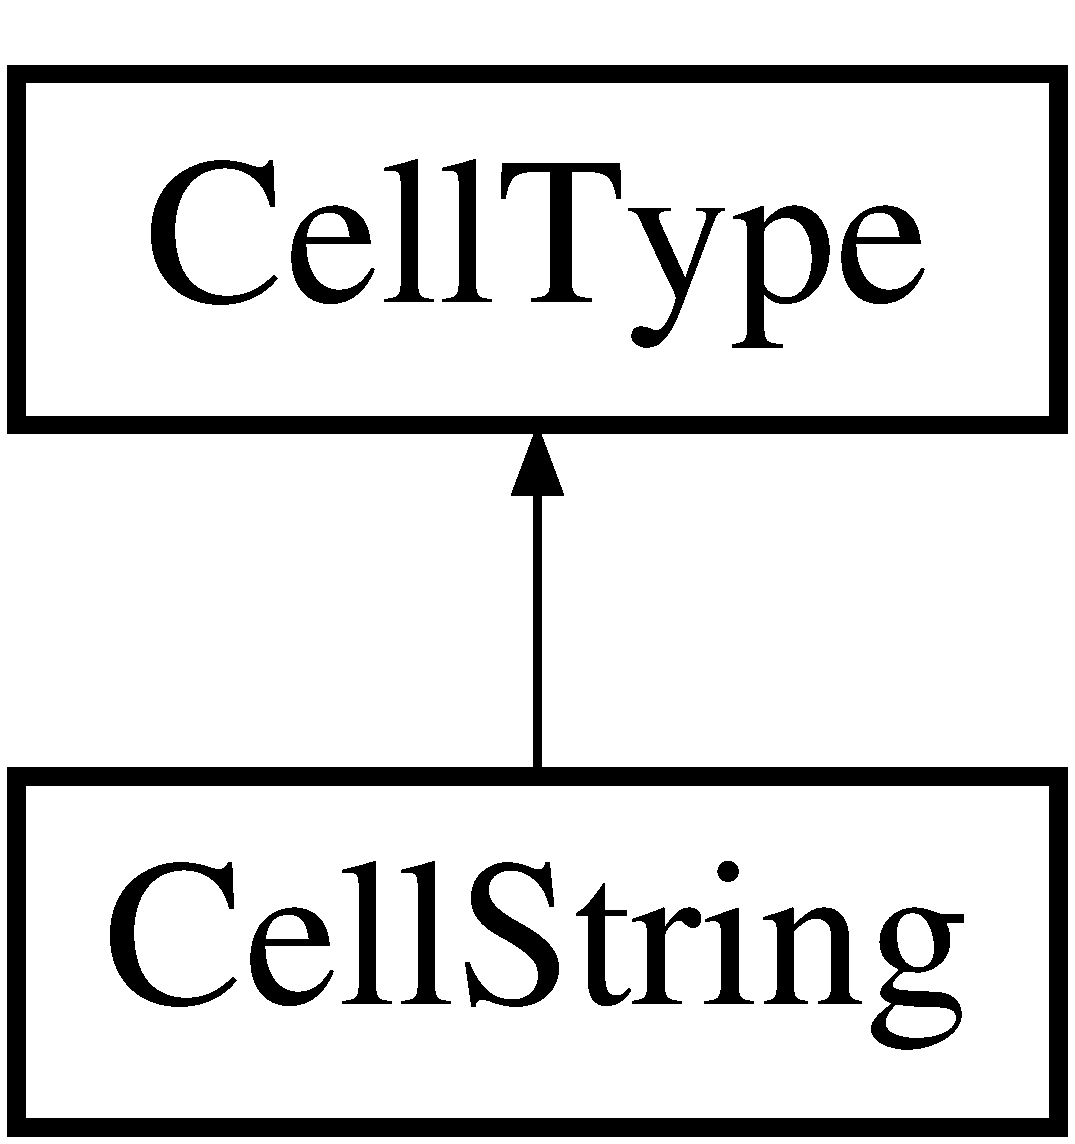
\includegraphics[height=2.000000cm]{class_cell_string}
\end{center}
\end{figure}
\subsection*{Public Member Functions}
\begin{DoxyCompactItemize}
\item 
\mbox{\Hypertarget{class_cell_string_a6a7bf500e09988f0de08ceeb9699fff9}\label{class_cell_string_a6a7bf500e09988f0de08ceeb9699fff9}} 
\hyperlink{class_cell_string_a6a7bf500e09988f0de08ceeb9699fff9}{Cell\+String} ()
\begin{DoxyCompactList}\small\item\em Default constructor. \end{DoxyCompactList}\item 
\mbox{\Hypertarget{class_cell_string_a6b310a8a51cca0a121ec497d4f954606}\label{class_cell_string_a6b310a8a51cca0a121ec497d4f954606}} 
\hyperlink{class_cell_string_a6b310a8a51cca0a121ec497d4f954606}{Cell\+String} (const \hyperlink{class_string}{String} rhs)
\begin{DoxyCompactList}\small\item\em Create new obj from \hyperlink{class_string}{String}. \end{DoxyCompactList}\item 
\mbox{\Hypertarget{class_cell_string_afbddebf6bfc5d2deb316a60141485724}\label{class_cell_string_afbddebf6bfc5d2deb316a60141485724}} 
\hyperlink{class_cell_string_afbddebf6bfc5d2deb316a60141485724}{Cell\+String} (const char $\ast$text)
\begin{DoxyCompactList}\small\item\em Create new obj from char array. \end{DoxyCompactList}\item 
\mbox{\Hypertarget{class_cell_string_a7381bd83019a62b33aac3d887da61b64}\label{class_cell_string_a7381bd83019a62b33aac3d887da61b64}} 
\hyperlink{class_cell_string_a7381bd83019a62b33aac3d887da61b64}{Cell\+String} (char symbol)
\begin{DoxyCompactList}\small\item\em Create new obj from single character. \end{DoxyCompactList}\item 
virtual \hyperlink{class_cell_type}{Cell\+Type} $\ast$ \hyperlink{class_cell_string_a293639128fa52df8f72f88335e23d2f0}{clone} () const
\item 
virtual void \hyperlink{class_cell_string_a13f416bd887f2cbceb93273316d16d65}{print} (std\+::ostream \&out) const
\item 
virtual unsigned \hyperlink{class_cell_string_a6a8f5570104283eb4bb8e9ed4b998fb7}{lenght} () const
\item 
virtual double \hyperlink{class_cell_string_a452054b2d80356d66ed7504d7b1b8d69}{value} () const
\item 
virtual \hyperlink{class_string}{String} \hyperlink{class_cell_string_a0670fd5a35f8e05c985379acd5e4b88f}{type} () const
\item 
virtual \hyperlink{class_string}{String} \hyperlink{class_cell_string_ac601c93ecb70391eae65236c56c561a5}{string\+Cell} () const
\end{DoxyCompactItemize}


\subsection{Detailed Description}
Class \hyperlink{class_cell_string}{Cell\+String} description. 

\hyperlink{class_string}{String} type of the cell derivated class at \hyperlink{class_cell_type}{Cell\+Type} The class value can be converted to a number if it\textquotesingle{}s content is valid number 

\subsection{Member Function Documentation}
\mbox{\Hypertarget{class_cell_string_a293639128fa52df8f72f88335e23d2f0}\label{class_cell_string_a293639128fa52df8f72f88335e23d2f0}} 
\index{Cell\+String@{Cell\+String}!clone@{clone}}
\index{clone@{clone}!Cell\+String@{Cell\+String}}
\subsubsection{\texorpdfstring{clone()}{clone()}}
{\footnotesize\ttfamily \hyperlink{class_cell_type}{Cell\+Type} $\ast$ Cell\+String\+::clone (\begin{DoxyParamCaption}{ }\end{DoxyParamCaption}) const\hspace{0.3cm}{\ttfamily [virtual]}}

Derivate class can be cloned -\/ Returns pointer to himself 

Implements \hyperlink{class_cell_type_a8c534b1eed27659429f761fc76d51b89}{Cell\+Type}.

\mbox{\Hypertarget{class_cell_string_a6a8f5570104283eb4bb8e9ed4b998fb7}\label{class_cell_string_a6a8f5570104283eb4bb8e9ed4b998fb7}} 
\index{Cell\+String@{Cell\+String}!lenght@{lenght}}
\index{lenght@{lenght}!Cell\+String@{Cell\+String}}
\subsubsection{\texorpdfstring{lenght()}{lenght()}}
{\footnotesize\ttfamily unsigned Cell\+String\+::lenght (\begin{DoxyParamCaption}{ }\end{DoxyParamCaption}) const\hspace{0.3cm}{\ttfamily [virtual]}}

Return lenght of the Cell type 

Implements \hyperlink{class_cell_type_a1f8bd268dbd474dd8e08726a6efac066}{Cell\+Type}.

\mbox{\Hypertarget{class_cell_string_a13f416bd887f2cbceb93273316d16d65}\label{class_cell_string_a13f416bd887f2cbceb93273316d16d65}} 
\index{Cell\+String@{Cell\+String}!print@{print}}
\index{print@{print}!Cell\+String@{Cell\+String}}
\subsubsection{\texorpdfstring{print()}{print()}}
{\footnotesize\ttfamily void Cell\+String\+::print (\begin{DoxyParamCaption}\item[{std\+::ostream \&}]{out }\end{DoxyParamCaption}) const\hspace{0.3cm}{\ttfamily [virtual]}}

Print on the stream given as the first argument 

Implements \hyperlink{class_cell_type_a34413fcb76f292b6b8d08615765ba894}{Cell\+Type}.

\mbox{\Hypertarget{class_cell_string_ac601c93ecb70391eae65236c56c561a5}\label{class_cell_string_ac601c93ecb70391eae65236c56c561a5}} 
\index{Cell\+String@{Cell\+String}!string\+Cell@{string\+Cell}}
\index{string\+Cell@{string\+Cell}!Cell\+String@{Cell\+String}}
\subsubsection{\texorpdfstring{string\+Cell()}{stringCell()}}
{\footnotesize\ttfamily \hyperlink{class_string}{String} Cell\+String\+::string\+Cell (\begin{DoxyParamCaption}{ }\end{DoxyParamCaption}) const\hspace{0.3cm}{\ttfamily [virtual]}}

Return a content of the cell 

Implements \hyperlink{class_cell_type_abba4d6d43efa340144d1ad09637e1aa9}{Cell\+Type}.

\mbox{\Hypertarget{class_cell_string_a0670fd5a35f8e05c985379acd5e4b88f}\label{class_cell_string_a0670fd5a35f8e05c985379acd5e4b88f}} 
\index{Cell\+String@{Cell\+String}!type@{type}}
\index{type@{type}!Cell\+String@{Cell\+String}}
\subsubsection{\texorpdfstring{type()}{type()}}
{\footnotesize\ttfamily \hyperlink{class_string}{String} Cell\+String\+::type (\begin{DoxyParamCaption}{ }\end{DoxyParamCaption}) const\hspace{0.3cm}{\ttfamily [virtual]}}

Return Cell type name 

Implements \hyperlink{class_cell_type_ae31acfe1efc7776796d85918886247af}{Cell\+Type}.

\mbox{\Hypertarget{class_cell_string_a452054b2d80356d66ed7504d7b1b8d69}\label{class_cell_string_a452054b2d80356d66ed7504d7b1b8d69}} 
\index{Cell\+String@{Cell\+String}!value@{value}}
\index{value@{value}!Cell\+String@{Cell\+String}}
\subsubsection{\texorpdfstring{value()}{value()}}
{\footnotesize\ttfamily double Cell\+String\+::value (\begin{DoxyParamCaption}{ }\end{DoxyParamCaption}) const\hspace{0.3cm}{\ttfamily [virtual]}}

Return value of the Cell type 

Implements \hyperlink{class_cell_type_a6cbfc477f605049f2a007d8674442230}{Cell\+Type}.



The documentation for this class was generated from the following files\+:\begin{DoxyCompactItemize}
\item 
D\+:/ФМИ/\+I\+I semestyr/\+O\+O\+P/fn45311 Spreadsheet project-\/updated/\+Project Speadsheets/Cell\+String.\+h\item 
D\+:/ФМИ/\+I\+I semestyr/\+O\+O\+P/fn45311 Spreadsheet project-\/updated/\+Project Speadsheets/Cell\+String.\+cpp\end{DoxyCompactItemize}

\hypertarget{class_cell_type}{}\section{Cell\+Type Class Reference}
\label{class_cell_type}\index{Cell\+Type@{Cell\+Type}}


Class \hyperlink{class_cell_type}{Cell\+Type} description.  




{\ttfamily \#include $<$Cell\+Type.\+h$>$}

Inheritance diagram for Cell\+Type\+:\begin{figure}[H]
\begin{center}
\leavevmode
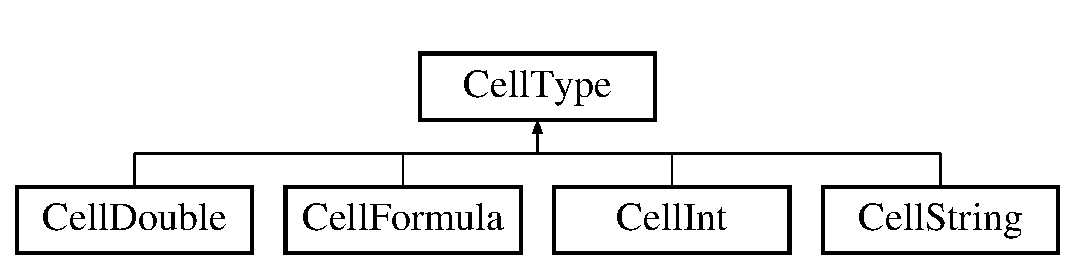
\includegraphics[height=2.000000cm]{class_cell_type}
\end{center}
\end{figure}
\subsection*{Public Member Functions}
\begin{DoxyCompactItemize}
\item 
virtual \hyperlink{class_cell_type}{Cell\+Type} $\ast$ \hyperlink{class_cell_type_a8c534b1eed27659429f761fc76d51b89}{clone} () const =0
\item 
virtual void \hyperlink{class_cell_type_a34413fcb76f292b6b8d08615765ba894}{print} (std\+::ostream \&out) const =0
\item 
virtual unsigned \hyperlink{class_cell_type_a1f8bd268dbd474dd8e08726a6efac066}{lenght} () const =0
\item 
virtual double \hyperlink{class_cell_type_a6cbfc477f605049f2a007d8674442230}{value} () const =0
\item 
virtual \hyperlink{class_string}{String} \hyperlink{class_cell_type_ae31acfe1efc7776796d85918886247af}{type} () const =0
\item 
virtual \hyperlink{class_string}{String} \hyperlink{class_cell_type_abba4d6d43efa340144d1ad09637e1aa9}{string\+Cell} () const =0
\end{DoxyCompactItemize}


\subsection{Detailed Description}
Class \hyperlink{class_cell_type}{Cell\+Type} description. 

Base class for the all Cell type pure virtual class 

\subsection{Member Function Documentation}
\mbox{\Hypertarget{class_cell_type_a8c534b1eed27659429f761fc76d51b89}\label{class_cell_type_a8c534b1eed27659429f761fc76d51b89}} 
\index{Cell\+Type@{Cell\+Type}!clone@{clone}}
\index{clone@{clone}!Cell\+Type@{Cell\+Type}}
\subsubsection{\texorpdfstring{clone()}{clone()}}
{\footnotesize\ttfamily virtual \hyperlink{class_cell_type}{Cell\+Type}$\ast$ Cell\+Type\+::clone (\begin{DoxyParamCaption}{ }\end{DoxyParamCaption}) const\hspace{0.3cm}{\ttfamily [pure virtual]}}

Derivate class can be cloned -\/ Returns pointer to himself 

Implemented in \hyperlink{class_cell_string_a293639128fa52df8f72f88335e23d2f0}{Cell\+String}, \hyperlink{class_cell_formula_a23c26c40ef7056d9395ed8bc4ebef3b9}{Cell\+Formula}, \hyperlink{class_cell_int_a767b15d99c5ec0e2594dc35300e51873}{Cell\+Int}, and \hyperlink{class_cell_double_a8d378687ae89338267e61d61ff932680}{Cell\+Double}.

\mbox{\Hypertarget{class_cell_type_a1f8bd268dbd474dd8e08726a6efac066}\label{class_cell_type_a1f8bd268dbd474dd8e08726a6efac066}} 
\index{Cell\+Type@{Cell\+Type}!lenght@{lenght}}
\index{lenght@{lenght}!Cell\+Type@{Cell\+Type}}
\subsubsection{\texorpdfstring{lenght()}{lenght()}}
{\footnotesize\ttfamily virtual unsigned Cell\+Type\+::lenght (\begin{DoxyParamCaption}{ }\end{DoxyParamCaption}) const\hspace{0.3cm}{\ttfamily [pure virtual]}}

Return lenght of the Cell type 

Implemented in \hyperlink{class_cell_string_a6a8f5570104283eb4bb8e9ed4b998fb7}{Cell\+String}, \hyperlink{class_cell_formula_af188e3f639245c126e0ae30e17b8d3c0}{Cell\+Formula}, \hyperlink{class_cell_int_afcab8270ff1853a08460051e02e62ace}{Cell\+Int}, and \hyperlink{class_cell_double_ac2d36517f1107fb0271172ea30d6bff5}{Cell\+Double}.

\mbox{\Hypertarget{class_cell_type_a34413fcb76f292b6b8d08615765ba894}\label{class_cell_type_a34413fcb76f292b6b8d08615765ba894}} 
\index{Cell\+Type@{Cell\+Type}!print@{print}}
\index{print@{print}!Cell\+Type@{Cell\+Type}}
\subsubsection{\texorpdfstring{print()}{print()}}
{\footnotesize\ttfamily virtual void Cell\+Type\+::print (\begin{DoxyParamCaption}\item[{std\+::ostream \&}]{out }\end{DoxyParamCaption}) const\hspace{0.3cm}{\ttfamily [pure virtual]}}

Print on the stream given as the first argument 

Implemented in \hyperlink{class_cell_string_a13f416bd887f2cbceb93273316d16d65}{Cell\+String}, \hyperlink{class_cell_formula_ac8cfeff2585811ee01acb7a4ddf25723}{Cell\+Formula}, \hyperlink{class_cell_int_a1cb8461721999308790d105adff41cd2}{Cell\+Int}, and \hyperlink{class_cell_double_a90539ceb6daa29e7b658d8f2a2d1445d}{Cell\+Double}.

\mbox{\Hypertarget{class_cell_type_abba4d6d43efa340144d1ad09637e1aa9}\label{class_cell_type_abba4d6d43efa340144d1ad09637e1aa9}} 
\index{Cell\+Type@{Cell\+Type}!string\+Cell@{string\+Cell}}
\index{string\+Cell@{string\+Cell}!Cell\+Type@{Cell\+Type}}
\subsubsection{\texorpdfstring{string\+Cell()}{stringCell()}}
{\footnotesize\ttfamily virtual \hyperlink{class_string}{String} Cell\+Type\+::string\+Cell (\begin{DoxyParamCaption}{ }\end{DoxyParamCaption}) const\hspace{0.3cm}{\ttfamily [pure virtual]}}

Return a content of the cell 

Implemented in \hyperlink{class_cell_string_ac601c93ecb70391eae65236c56c561a5}{Cell\+String}, \hyperlink{class_cell_formula_abe70a7ace4b58fe4154bacccb5e3c12c}{Cell\+Formula}, \hyperlink{class_cell_int_ae6b32857bc96f305fff4226c988032d4}{Cell\+Int}, and \hyperlink{class_cell_double_a3e92f9ec4b564b3e14fa829529bbaf0a}{Cell\+Double}.

\mbox{\Hypertarget{class_cell_type_ae31acfe1efc7776796d85918886247af}\label{class_cell_type_ae31acfe1efc7776796d85918886247af}} 
\index{Cell\+Type@{Cell\+Type}!type@{type}}
\index{type@{type}!Cell\+Type@{Cell\+Type}}
\subsubsection{\texorpdfstring{type()}{type()}}
{\footnotesize\ttfamily virtual \hyperlink{class_string}{String} Cell\+Type\+::type (\begin{DoxyParamCaption}{ }\end{DoxyParamCaption}) const\hspace{0.3cm}{\ttfamily [pure virtual]}}

Return Cell type name 

Implemented in \hyperlink{class_cell_string_a0670fd5a35f8e05c985379acd5e4b88f}{Cell\+String}, \hyperlink{class_cell_formula_ae175fd79ee036efa3a968f37b8eb53bc}{Cell\+Formula}, \hyperlink{class_cell_int_a65c7fa9731cc6f5b40579f314ba090dd}{Cell\+Int}, and \hyperlink{class_cell_double_a73662d15e8626c81858e3a243f0d6818}{Cell\+Double}.

\mbox{\Hypertarget{class_cell_type_a6cbfc477f605049f2a007d8674442230}\label{class_cell_type_a6cbfc477f605049f2a007d8674442230}} 
\index{Cell\+Type@{Cell\+Type}!value@{value}}
\index{value@{value}!Cell\+Type@{Cell\+Type}}
\subsubsection{\texorpdfstring{value()}{value()}}
{\footnotesize\ttfamily virtual double Cell\+Type\+::value (\begin{DoxyParamCaption}{ }\end{DoxyParamCaption}) const\hspace{0.3cm}{\ttfamily [pure virtual]}}

Return value of the Cell type 

Implemented in \hyperlink{class_cell_string_a452054b2d80356d66ed7504d7b1b8d69}{Cell\+String}, \hyperlink{class_cell_formula_a29d9e3000ae3f0b0ebac72807a455fec}{Cell\+Formula}, \hyperlink{class_cell_int_a1be32d235fbcc58483948770fb7ce9c6}{Cell\+Int}, and \hyperlink{class_cell_double_a6ed39c7b32c0599b4db0f046c7cfab93}{Cell\+Double}.



The documentation for this class was generated from the following files\+:\begin{DoxyCompactItemize}
\item 
D\+:/ФМИ/\+I\+I semestyr/\+O\+O\+P/fn45311 Spreadsheet project-\/updated/\+Project Speadsheets/Cell\+Type.\+h\item 
D\+:/ФМИ/\+I\+I semestyr/\+O\+O\+P/fn45311 Spreadsheet project-\/updated/\+Project Speadsheets/Cell\+Type.\+cpp\end{DoxyCompactItemize}

\hypertarget{class_command}{}\section{Command Class Reference}
\label{class_command}\index{Command@{Command}}


Class \hyperlink{class_command}{Command} description.  




{\ttfamily \#include $<$Command.\+h$>$}

\subsection*{Public Member Functions}
\begin{DoxyCompactItemize}
\item 
\mbox{\Hypertarget{class_command_a18df2d81039392daeb0b78c346a70537}\label{class_command_a18df2d81039392daeb0b78c346a70537}} 
\hyperlink{class_command_a18df2d81039392daeb0b78c346a70537}{Command} ()
\begin{DoxyCompactList}\small\item\em Default constructor. \end{DoxyCompactList}\item 
\mbox{\Hypertarget{class_command_a28004856f059802e3016c780c80e5181}\label{class_command_a28004856f059802e3016c780c80e5181}} 
\hyperlink{class_command_a28004856f059802e3016c780c80e5181}{Command} (const \hyperlink{class_command}{Command} \&rhs)
\begin{DoxyCompactList}\small\item\em Copy constructor. \end{DoxyCompactList}\item 
\mbox{\Hypertarget{class_command_a7a1d6c31ddfc1ab65453a93de293be4e}\label{class_command_a7a1d6c31ddfc1ab65453a93de293be4e}} 
\hyperlink{class_command_a7a1d6c31ddfc1ab65453a93de293be4e}{Command} (const \hyperlink{class_string}{String} text)
\begin{DoxyCompactList}\small\item\em Create new obj from \hyperlink{class_string}{String}. \end{DoxyCompactList}\item 
\mbox{\Hypertarget{class_command_a7d6b48fcb77bbbc99d7661cce384d8dc}\label{class_command_a7d6b48fcb77bbbc99d7661cce384d8dc}} 
\hyperlink{class_command_a7d6b48fcb77bbbc99d7661cce384d8dc}{Command} (const char $\ast$text)
\begin{DoxyCompactList}\small\item\em Create new obj from char array. \end{DoxyCompactList}\item 
\mbox{\Hypertarget{class_command_ac86295c87439d6e845bb47e702be5e9e}\label{class_command_ac86295c87439d6e845bb47e702be5e9e}} 
\hyperlink{class_command_ac86295c87439d6e845bb47e702be5e9e}{Command} (const char symbol)
\begin{DoxyCompactList}\small\item\em Create new obj from single character. \end{DoxyCompactList}\item 
\mbox{\Hypertarget{class_command_ab552bb3a07fdd1acbfd8ea76e69b2278}\label{class_command_ab552bb3a07fdd1acbfd8ea76e69b2278}} 
\hyperlink{class_command_ab552bb3a07fdd1acbfd8ea76e69b2278}{$\sim$\+Command} ()
\begin{DoxyCompactList}\small\item\em Destructor. \end{DoxyCompactList}\item 
\mbox{\Hypertarget{class_command_a6f283aa5560e5e044b53aa1f5739d7ed}\label{class_command_a6f283aa5560e5e044b53aa1f5739d7ed}} 
\hyperlink{class_command}{Command} \& \hyperlink{class_command_a6f283aa5560e5e044b53aa1f5739d7ed}{operator=} (const \hyperlink{class_command}{Command} \&rhs)
\begin{DoxyCompactList}\small\item\em Assign from \hyperlink{class_command}{Command} obj. \end{DoxyCompactList}\item 
\mbox{\Hypertarget{class_command_a8b6fd56b6bbcc598523ab947367720c1}\label{class_command_a8b6fd56b6bbcc598523ab947367720c1}} 
\hyperlink{class_command}{Command} \& \hyperlink{class_command_a8b6fd56b6bbcc598523ab947367720c1}{operator=} (const \hyperlink{class_string}{String} \&rhs)
\begin{DoxyCompactList}\small\item\em Assign from \hyperlink{class_string}{String}. \end{DoxyCompactList}\item 
\mbox{\Hypertarget{class_command_a7fa1e89e5a4aa8fed864046f20db1a3b}\label{class_command_a7fa1e89e5a4aa8fed864046f20db1a3b}} 
\hyperlink{class_command}{Command} \& \hyperlink{class_command_a7fa1e89e5a4aa8fed864046f20db1a3b}{operator=} (const char $\ast$rhs)
\begin{DoxyCompactList}\small\item\em Assign from char array. \end{DoxyCompactList}\item 
\mbox{\Hypertarget{class_command_ab9b317d3af1cb59a7c402b9a41b7f624}\label{class_command_ab9b317d3af1cb59a7c402b9a41b7f624}} 
\hyperlink{class_command}{Command} \& \hyperlink{class_command_ab9b317d3af1cb59a7c402b9a41b7f624}{operator=} (char symbol)
\begin{DoxyCompactList}\small\item\em Assign from signle character. \end{DoxyCompactList}\item 
\mbox{\Hypertarget{class_command_aff1c77698af9ba96ece3c7e98d83b0e5}\label{class_command_aff1c77698af9ba96ece3c7e98d83b0e5}} 
\hyperlink{class_string}{String} \hyperlink{class_command_aff1c77698af9ba96ece3c7e98d83b0e5}{task} () const
\begin{DoxyCompactList}\small\item\em Return command task. \end{DoxyCompactList}\item 
\mbox{\Hypertarget{class_command_a52a3124585505db25a55fc54d7aec603}\label{class_command_a52a3124585505db25a55fc54d7aec603}} 
\hyperlink{class_string}{String} \hyperlink{class_command_a52a3124585505db25a55fc54d7aec603}{command\+Arg} () const
\begin{DoxyCompactList}\small\item\em Return command argument. \end{DoxyCompactList}\item 
\mbox{\Hypertarget{class_command_a57fbea0c0d10ef4b184c7ef3eb34590d}\label{class_command_a57fbea0c0d10ef4b184c7ef3eb34590d}} 
void \hyperlink{class_command_a57fbea0c0d10ef4b184c7ef3eb34590d}{clear} ()
\begin{DoxyCompactList}\small\item\em Clear command task and argument. \end{DoxyCompactList}\item 
void \hyperlink{class_command_a9209fc53d344c17fe39e27a3ef5d566f}{set} (const \hyperlink{class_string}{String} text)
\item 
\mbox{\Hypertarget{class_command_aa13e98e5f35773b360931da7ac6ca504}\label{class_command_aa13e98e5f35773b360931da7ac6ca504}} 
void {\bfseries set} (const char $\ast$text)
\item 
\mbox{\Hypertarget{class_command_a73871dc74261367bb8423544018e8d8d}\label{class_command_a73871dc74261367bb8423544018e8d8d}} 
void {\bfseries set} (const char symbol)
\item 
void \hyperlink{class_command_a90eaeb4bfb180ca4cafa61db2b3e0677}{execute} () const
\begin{DoxyCompactList}\small\item\em Execute the \hyperlink{class_spreadsheet}{Spreadsheet} command. \end{DoxyCompactList}\end{DoxyCompactItemize}


\subsection{Detailed Description}
Class \hyperlink{class_command}{Command} description. 

Convert \hyperlink{class_string}{String} into \hyperlink{class_spreadsheet}{Spreadsheet} command task and command argument and execute the command



 \hyperlink{class_spreadsheet}{Spreadsheet} support only a comma-\/separated values (C\+SV) files.

Available \hyperlink{class_spreadsheet}{Spreadsheet} commands\+:
\begin{DoxyItemize}
\item open $<$\+Path\+To\+File$>$ -\/ Open specified file, given as the first argument. If the file does not exist then it\textquotesingle{}s been created.
\item close -\/ Closes an already opened file without saving any changes in it. Close does not exit the program. If no file has been opened, you get an E\+R\+R\+OR.
\item save -\/ Saves data in the opened file. If no file has been opened, you get an E\+R\+R\+OR.
\item saveas $<$\+Path\+To\+File$>$ -\/ Saves data in the specified file, given as the first argument. If no file has been opened, you get an E\+R\+R\+OR.
\item print -\/ Prints files data on console window. If no file has been opened, you get an E\+R\+R\+OR.
\item edit R$<$value$>$C$<$value$>$ $<$\+New\+Cell\+Value$>$ -\/ Changes value in given cell. First argument specifies row and column of the cell. Second argument specifies the new cell value. Valids data types are\+: $<$integer$>$, $<$double$>$, "$<$string$>$", =$<$formula$>$.
\item add \mbox{[}row$\vert$col\mbox{]} $<$unsigned$>$ -\/ Add empty row or column. Second argument specifies the number of the new rows or columns.
\item exit -\/ Exit the program without saving any changes in opened file, if there is one.
\item help -\/ Prints available commands info. 
\end{DoxyItemize}

\subsection{Member Function Documentation}
\mbox{\Hypertarget{class_command_a90eaeb4bfb180ca4cafa61db2b3e0677}\label{class_command_a90eaeb4bfb180ca4cafa61db2b3e0677}} 
\index{Command@{Command}!execute@{execute}}
\index{execute@{execute}!Command@{Command}}
\subsubsection{\texorpdfstring{execute()}{execute()}}
{\footnotesize\ttfamily void Command\+::execute (\begin{DoxyParamCaption}{ }\end{DoxyParamCaption}) const}



Execute the \hyperlink{class_spreadsheet}{Spreadsheet} command. 

Execute \hyperlink{class_command}{Command}. \mbox{\Hypertarget{class_command_a9209fc53d344c17fe39e27a3ef5d566f}\label{class_command_a9209fc53d344c17fe39e27a3ef5d566f}} 
\index{Command@{Command}!set@{set}}
\index{set@{set}!Command@{Command}}
\subsubsection{\texorpdfstring{set()}{set()}}
{\footnotesize\ttfamily void Command\+::set (\begin{DoxyParamCaption}\item[{const \hyperlink{class_string}{String}}]{text }\end{DoxyParamCaption})}

Set \hyperlink{class_command}{Command} values from different sources 

The documentation for this class was generated from the following files\+:\begin{DoxyCompactItemize}
\item 
D\+:/ФМИ/\+I\+I semestyr/\+O\+O\+P/fn45311 Spreadsheet project-\/updated/\+Project Speadsheets/Command.\+h\item 
D\+:/ФМИ/\+I\+I semestyr/\+O\+O\+P/fn45311 Spreadsheet project-\/updated/\+Project Speadsheets/Command.\+cpp\end{DoxyCompactItemize}

\hypertarget{class_spreadsheet}{}\section{Spreadsheet Class Reference}
\label{class_spreadsheet}\index{Spreadsheet@{Spreadsheet}}


Class \hyperlink{class_spreadsheet}{Spreadsheet} description.  




{\ttfamily \#include $<$Speadsheet.\+h$>$}

\subsection*{Public Member Functions}
\begin{DoxyCompactItemize}
\item 
\mbox{\Hypertarget{class_spreadsheet_ac2cd7c97b5d73805edcd14891d910f51}\label{class_spreadsheet_ac2cd7c97b5d73805edcd14891d910f51}} 
unsigned \hyperlink{class_spreadsheet_ac2cd7c97b5d73805edcd14891d910f51}{row} () const
\begin{DoxyCompactList}\small\item\em Get number of rows in the \hyperlink{class_spreadsheet}{Spreadsheet}. \end{DoxyCompactList}\item 
\mbox{\Hypertarget{class_spreadsheet_abee8b54fceb0f2c4314bbaf624feed75}\label{class_spreadsheet_abee8b54fceb0f2c4314bbaf624feed75}} 
unsigned \hyperlink{class_spreadsheet_abee8b54fceb0f2c4314bbaf624feed75}{col} () const
\begin{DoxyCompactList}\small\item\em Get number of columns in the \hyperlink{class_spreadsheet}{Spreadsheet}. \end{DoxyCompactList}\item 
\mbox{\Hypertarget{class_spreadsheet_a29e1c16f68d43f5ce96c15f1c18c71de}\label{class_spreadsheet_a29e1c16f68d43f5ce96c15f1c18c71de}} 
\hyperlink{class_string}{String} \hyperlink{class_spreadsheet_a29e1c16f68d43f5ce96c15f1c18c71de}{file\+Name} () const
\begin{DoxyCompactList}\small\item\em Get file name of the \hyperlink{class_spreadsheet}{Spreadsheet} if is open. \end{DoxyCompactList}\item 
\mbox{\Hypertarget{class_spreadsheet_a4c8bab95a22c86d5a8a75e54a7e82c51}\label{class_spreadsheet_a4c8bab95a22c86d5a8a75e54a7e82c51}} 
bool \hyperlink{class_spreadsheet_a4c8bab95a22c86d5a8a75e54a7e82c51}{is\+Open} () const
\begin{DoxyCompactList}\small\item\em Get information if the \hyperlink{class_spreadsheet}{Spreadsheet} is open. \end{DoxyCompactList}\item 
\mbox{\Hypertarget{class_spreadsheet_aa46282ef1877328ccc2626791dbc7cdf}\label{class_spreadsheet_aa46282ef1877328ccc2626791dbc7cdf}} 
unsigned \hyperlink{class_spreadsheet_aa46282ef1877328ccc2626791dbc7cdf}{get\+Cell\+Lenght} (unsigned index) const
\begin{DoxyCompactList}\small\item\em Get max\+Cell lenght. \end{DoxyCompactList}\item 
\mbox{\Hypertarget{class_spreadsheet_a6d920dbf2f30f6c69955fd0d1a3980db}\label{class_spreadsheet_a6d920dbf2f30f6c69955fd0d1a3980db}} 
const \hyperlink{class_cell_type}{Cell\+Type} $\ast$ \hyperlink{class_spreadsheet_a6d920dbf2f30f6c69955fd0d1a3980db}{operator\mbox{[}$\,$\mbox{]}} (\hyperlink{class_string}{String} arg) const
\begin{DoxyCompactList}\small\item\em Take cell R$<$value$>$C$<$value$>$ \end{DoxyCompactList}\item 
\mbox{\Hypertarget{class_spreadsheet_a85df209927f0e389fdb0a4528c62a29f}\label{class_spreadsheet_a85df209927f0e389fdb0a4528c62a29f}} 
\hyperlink{class_cell_type}{Cell\+Type} $\ast$ {\bfseries operator\mbox{[}$\,$\mbox{]}} (\hyperlink{class_string}{String} arg)
\item 
\mbox{\Hypertarget{class_spreadsheet_ad0befef369800a0f0f4b631c8ff96769}\label{class_spreadsheet_ad0befef369800a0f0f4b631c8ff96769}} 
const \hyperlink{class_cell_type}{Cell\+Type} $\ast$ \hyperlink{class_spreadsheet_ad0befef369800a0f0f4b631c8ff96769}{take\+Cell} (unsigned \hyperlink{class_spreadsheet_ac2cd7c97b5d73805edcd14891d910f51}{row}, unsigned \hyperlink{class_spreadsheet_abee8b54fceb0f2c4314bbaf624feed75}{col}) const
\begin{DoxyCompactList}\small\item\em Take cell. \end{DoxyCompactList}\item 
bool \hyperlink{class_spreadsheet_a541ce5ddde2c929e67230042434f4d07}{is\+Valid\+Cell} (const \hyperlink{class_string}{String} data) const
\item 
void \hyperlink{class_spreadsheet_a8183b9507cf53567b831352f27350688}{set\+Cells} (\hyperlink{class_cell_type}{Cell\+Type} $\ast$$\ast$$\ast$cells, unsigned row\+Size, unsigned col\+Size)
\begin{DoxyCompactList}\small\item\em Set Cells, row and col size, and max colum lenght. \end{DoxyCompactList}\item 
\mbox{\Hypertarget{class_spreadsheet_a0bf601cc24e9a3cc62a116e1e8e3a74f}\label{class_spreadsheet_a0bf601cc24e9a3cc62a116e1e8e3a74f}} 
void \hyperlink{class_spreadsheet_a0bf601cc24e9a3cc62a116e1e8e3a74f}{change\+Cell} (\hyperlink{class_string}{String} index, \hyperlink{class_cell_type}{Cell\+Type} $\ast$new\+Value)
\begin{DoxyCompactList}\small\item\em Change single cell value and type. \end{DoxyCompactList}\item 
\mbox{\Hypertarget{class_spreadsheet_a24589d9a703aa835682bf3222e944ddb}\label{class_spreadsheet_a24589d9a703aa835682bf3222e944ddb}} 
void \hyperlink{class_spreadsheet_a24589d9a703aa835682bf3222e944ddb}{set\+File\+Name} (\hyperlink{class_string}{String} \hyperlink{class_spreadsheet_a29e1c16f68d43f5ce96c15f1c18c71de}{file\+Name})
\begin{DoxyCompactList}\small\item\em Set \hyperlink{class_spreadsheet}{Spreadsheet} file name. \end{DoxyCompactList}\item 
\mbox{\Hypertarget{class_spreadsheet_aa3a53ae9bccfcaf880465198dc7f4e33}\label{class_spreadsheet_aa3a53ae9bccfcaf880465198dc7f4e33}} 
void \hyperlink{class_spreadsheet_aa3a53ae9bccfcaf880465198dc7f4e33}{set\+Is\+Open} (bool \hyperlink{class_spreadsheet_a4c8bab95a22c86d5a8a75e54a7e82c51}{is\+Open})
\begin{DoxyCompactList}\small\item\em Set if the \hyperlink{class_spreadsheet}{Spreadsheet} is open. \end{DoxyCompactList}\item 
void \hyperlink{class_spreadsheet_a5c0f7b4ebd4da1741a662fe595f32cbc}{clean} ()
\begin{DoxyCompactList}\small\item\em Clean the \hyperlink{class_spreadsheet}{Spreadsheet} values. \end{DoxyCompactList}\end{DoxyCompactItemize}
\subsection*{Static Public Member Functions}
\begin{DoxyCompactItemize}
\item 
\mbox{\Hypertarget{class_spreadsheet_a128c4e331142e6e5bad870cb5b2e1917}\label{class_spreadsheet_a128c4e331142e6e5bad870cb5b2e1917}} 
static \hyperlink{class_spreadsheet}{Spreadsheet} \& \hyperlink{class_spreadsheet_a128c4e331142e6e5bad870cb5b2e1917}{get\+Instance} ()
\begin{DoxyCompactList}\small\item\em Get the pointer of the \hyperlink{class_spreadsheet}{Spreadsheet} obj. \end{DoxyCompactList}\item 
\mbox{\Hypertarget{class_spreadsheet_aa7ca5fb8133d735022684dc11271c71a}\label{class_spreadsheet_aa7ca5fb8133d735022684dc11271c71a}} 
static void \hyperlink{class_spreadsheet_aa7ca5fb8133d735022684dc11271c71a}{release} ()
\begin{DoxyCompactList}\small\item\em Release the pointer of the \hyperlink{class_spreadsheet}{Spreadsheet} obj. \end{DoxyCompactList}\end{DoxyCompactItemize}


\subsection{Detailed Description}
Class \hyperlink{class_spreadsheet}{Spreadsheet} description. 

\hyperlink{class_spreadsheet}{Spreadsheet} is Singleton obj. It have\+:
\begin{DoxyItemize}
\item cells with position R$<$value$>$C$<$value$>$ and different type\+: int, double, string and formula.
\item file name 
\end{DoxyItemize}

\subsection{Member Function Documentation}
\mbox{\Hypertarget{class_spreadsheet_a5c0f7b4ebd4da1741a662fe595f32cbc}\label{class_spreadsheet_a5c0f7b4ebd4da1741a662fe595f32cbc}} 
\index{Spreadsheet@{Spreadsheet}!clean@{clean}}
\index{clean@{clean}!Spreadsheet@{Spreadsheet}}
\subsubsection{\texorpdfstring{clean()}{clean()}}
{\footnotesize\ttfamily void Spreadsheet\+::clean (\begin{DoxyParamCaption}{ }\end{DoxyParamCaption})}



Clean the \hyperlink{class_spreadsheet}{Spreadsheet} values. 

Clean the \hyperlink{class_spreadsheet}{Spreadsheet} values \mbox{\Hypertarget{class_spreadsheet_a541ce5ddde2c929e67230042434f4d07}\label{class_spreadsheet_a541ce5ddde2c929e67230042434f4d07}} 
\index{Spreadsheet@{Spreadsheet}!is\+Valid\+Cell@{is\+Valid\+Cell}}
\index{is\+Valid\+Cell@{is\+Valid\+Cell}!Spreadsheet@{Spreadsheet}}
\subsubsection{\texorpdfstring{is\+Valid\+Cell()}{isValidCell()}}
{\footnotesize\ttfamily bool Spreadsheet\+::is\+Valid\+Cell (\begin{DoxyParamCaption}\item[{const \hyperlink{class_string}{String}}]{data }\end{DoxyParamCaption}) const}

Chech if this input is with valid data\+: R$<$value$>$C$<$value$>$ \mbox{\Hypertarget{class_spreadsheet_a8183b9507cf53567b831352f27350688}\label{class_spreadsheet_a8183b9507cf53567b831352f27350688}} 
\index{Spreadsheet@{Spreadsheet}!set\+Cells@{set\+Cells}}
\index{set\+Cells@{set\+Cells}!Spreadsheet@{Spreadsheet}}
\subsubsection{\texorpdfstring{set\+Cells()}{setCells()}}
{\footnotesize\ttfamily void Spreadsheet\+::set\+Cells (\begin{DoxyParamCaption}\item[{\hyperlink{class_cell_type}{Cell\+Type} $\ast$$\ast$$\ast$}]{cells,  }\item[{unsigned}]{row\+Size,  }\item[{unsigned}]{col\+Size }\end{DoxyParamCaption})}



Set Cells, row and col size, and max colum lenght. 

All set functions. Reset buffer Max\+Data\+Lenght 

The documentation for this class was generated from the following files\+:\begin{DoxyCompactItemize}
\item 
D\+:/ФМИ/\+I\+I semestyr/\+O\+O\+P/fn45311 Spreadsheet project-\/updated/\+Project Speadsheets/Speadsheet.\+h\item 
D\+:/ФМИ/\+I\+I semestyr/\+O\+O\+P/fn45311 Spreadsheet project-\/updated/\+Project Speadsheets/Speadsheet.\+cpp\end{DoxyCompactItemize}

\hypertarget{class_string}{}\section{String Class Reference}
\label{class_string}\index{String@{String}}


Class \hyperlink{class_string}{String} description.  




{\ttfamily \#include $<$String.\+h$>$}

\subsection*{Public Member Functions}
\begin{DoxyCompactItemize}
\item 
\mbox{\Hypertarget{class_string_a8a7ef356e05eb9b1ea1ab518baee3095}\label{class_string_a8a7ef356e05eb9b1ea1ab518baee3095}} 
\hyperlink{class_string_a8a7ef356e05eb9b1ea1ab518baee3095}{String} ()
\begin{DoxyCompactList}\small\item\em Default constructor. \end{DoxyCompactList}\item 
\mbox{\Hypertarget{class_string_a117f8a4ef8cd2c6b3632324b0146d7ae}\label{class_string_a117f8a4ef8cd2c6b3632324b0146d7ae}} 
\hyperlink{class_string_a117f8a4ef8cd2c6b3632324b0146d7ae}{String} (const \hyperlink{class_string}{String} \&rhs)
\begin{DoxyCompactList}\small\item\em Copy constructor. \end{DoxyCompactList}\item 
\mbox{\Hypertarget{class_string_a536209bdc6da85c29369073bed2bfd45}\label{class_string_a536209bdc6da85c29369073bed2bfd45}} 
\hyperlink{class_string_a536209bdc6da85c29369073bed2bfd45}{String} (const char $\ast$text)
\begin{DoxyCompactList}\small\item\em Construct string object from char array. \end{DoxyCompactList}\item 
\mbox{\Hypertarget{class_string_a8c3550b6c85fb4925d8afa67a6fdc867}\label{class_string_a8c3550b6c85fb4925d8afa67a6fdc867}} 
\hyperlink{class_string_a8c3550b6c85fb4925d8afa67a6fdc867}{String} (char symbol)
\begin{DoxyCompactList}\small\item\em Construct string object from character. \end{DoxyCompactList}\item 
\mbox{\Hypertarget{class_string_ac40b2a3fb58c2d8556f5e6ff73510036}\label{class_string_ac40b2a3fb58c2d8556f5e6ff73510036}} 
\hyperlink{class_string_ac40b2a3fb58c2d8556f5e6ff73510036}{$\sim$\+String} ()
\begin{DoxyCompactList}\small\item\em \hyperlink{class_string}{String} destructor. \end{DoxyCompactList}\item 
\mbox{\Hypertarget{class_string_a70b3aba8ac7a57e3bb48a52a5d64a88b}\label{class_string_a70b3aba8ac7a57e3bb48a52a5d64a88b}} 
\hyperlink{class_string}{String} \& \hyperlink{class_string_a70b3aba8ac7a57e3bb48a52a5d64a88b}{operator=} (const \hyperlink{class_string}{String} \&rhs)
\begin{DoxyCompactList}\small\item\em \hyperlink{class_string}{String} assignment from another \hyperlink{class_string}{String} obj. \end{DoxyCompactList}\item 
\mbox{\Hypertarget{class_string_adddd36a0442459193abb9562efa94886}\label{class_string_adddd36a0442459193abb9562efa94886}} 
\hyperlink{class_string}{String} \& \hyperlink{class_string_adddd36a0442459193abb9562efa94886}{operator=} (const char $\ast$rhs)
\begin{DoxyCompactList}\small\item\em \hyperlink{class_string}{String} assignment from char array. \end{DoxyCompactList}\item 
\mbox{\Hypertarget{class_string_a5015638c6c8bf1ae313608b89d194788}\label{class_string_a5015638c6c8bf1ae313608b89d194788}} 
\hyperlink{class_string}{String} \& \hyperlink{class_string_a5015638c6c8bf1ae313608b89d194788}{operator=} (char symbol)
\begin{DoxyCompactList}\small\item\em \hyperlink{class_string}{String} assignment from single character. \end{DoxyCompactList}\item 
\mbox{\Hypertarget{class_string_a77a7c0ae567c65fb98914a1beccfb337}\label{class_string_a77a7c0ae567c65fb98914a1beccfb337}} 
void \hyperlink{class_string_a77a7c0ae567c65fb98914a1beccfb337}{set} (const \hyperlink{class_string}{String} \&rhs)
\begin{DoxyCompactList}\small\item\em Set obj with value another \hyperlink{class_string}{String} obj. \end{DoxyCompactList}\item 
\mbox{\Hypertarget{class_string_a6ad3d14b203c5b4965804f2954b49bc9}\label{class_string_a6ad3d14b203c5b4965804f2954b49bc9}} 
void \hyperlink{class_string_a6ad3d14b203c5b4965804f2954b49bc9}{set} (const char $\ast$text)
\begin{DoxyCompactList}\small\item\em Set obj with value char array. \end{DoxyCompactList}\item 
\mbox{\Hypertarget{class_string_aadd64103fed706695d33dc3642389e3a}\label{class_string_aadd64103fed706695d33dc3642389e3a}} 
void \hyperlink{class_string_aadd64103fed706695d33dc3642389e3a}{set} (char symbol)
\begin{DoxyCompactList}\small\item\em Set obj with value single character. \end{DoxyCompactList}\item 
\mbox{\Hypertarget{class_string_a946016b80317f9b31982b0b12992654a}\label{class_string_a946016b80317f9b31982b0b12992654a}} 
unsigned \hyperlink{class_string_a946016b80317f9b31982b0b12992654a}{lenght} () const
\begin{DoxyCompactList}\small\item\em Return length of \hyperlink{class_string}{String}. \end{DoxyCompactList}\item 
\mbox{\Hypertarget{class_string_acf604fddaddc57ee1575b34ec1c1589d}\label{class_string_acf604fddaddc57ee1575b34ec1c1589d}} 
bool \hyperlink{class_string_acf604fddaddc57ee1575b34ec1c1589d}{empty} () const
\begin{DoxyCompactList}\small\item\em Test if string is empty. \end{DoxyCompactList}\item 
\mbox{\Hypertarget{class_string_ab5b0c43ae84247df8e5f9488a911587c}\label{class_string_ab5b0c43ae84247df8e5f9488a911587c}} 
void \hyperlink{class_string_ab5b0c43ae84247df8e5f9488a911587c}{clear} ()
\begin{DoxyCompactList}\small\item\em Clear string. \end{DoxyCompactList}\item 
\mbox{\Hypertarget{class_string_af1df131318966ea0bba5c6f603734600}\label{class_string_af1df131318966ea0bba5c6f603734600}} 
char \& \hyperlink{class_string_af1df131318966ea0bba5c6f603734600}{operator\mbox{[}$\,$\mbox{]}} (size\+\_\+t index)
\begin{DoxyCompactList}\small\item\em Get character of string. \end{DoxyCompactList}\item 
\mbox{\Hypertarget{class_string_a433ce8bc2e88d07f1865419fbf770ca5}\label{class_string_a433ce8bc2e88d07f1865419fbf770ca5}} 
const char \& \hyperlink{class_string_a433ce8bc2e88d07f1865419fbf770ca5}{operator\mbox{[}$\,$\mbox{]}} (size\+\_\+t index) const
\begin{DoxyCompactList}\small\item\em Get character of string. \end{DoxyCompactList}\item 
\mbox{\Hypertarget{class_string_a9c2c3075f6a490ef112e7f83e6cde351}\label{class_string_a9c2c3075f6a490ef112e7f83e6cde351}} 
char \& \hyperlink{class_string_a9c2c3075f6a490ef112e7f83e6cde351}{at} (size\+\_\+t index)
\begin{DoxyCompactList}\small\item\em Get character in string. \end{DoxyCompactList}\item 
\mbox{\Hypertarget{class_string_a3b3b3427a4a75888ee3812ea107fb9c6}\label{class_string_a3b3b3427a4a75888ee3812ea107fb9c6}} 
const char \& \hyperlink{class_string_a3b3b3427a4a75888ee3812ea107fb9c6}{at} (size\+\_\+t index) const
\begin{DoxyCompactList}\small\item\em Get character in string. \end{DoxyCompactList}\item 
\mbox{\Hypertarget{class_string_abb80e1189595b12b7466d7e38bde3b7c}\label{class_string_abb80e1189595b12b7466d7e38bde3b7c}} 
char \& \hyperlink{class_string_abb80e1189595b12b7466d7e38bde3b7c}{back} ()
\begin{DoxyCompactList}\small\item\em Access last character. \end{DoxyCompactList}\item 
\mbox{\Hypertarget{class_string_ac7c01a0e930f9381db72a879ddf05df2}\label{class_string_ac7c01a0e930f9381db72a879ddf05df2}} 
const char \& \hyperlink{class_string_ac7c01a0e930f9381db72a879ddf05df2}{back} () const
\begin{DoxyCompactList}\small\item\em Access last character. \end{DoxyCompactList}\item 
\mbox{\Hypertarget{class_string_ae5c8caa50e19cea1e6ac6e1666e7f5bd}\label{class_string_ae5c8caa50e19cea1e6ac6e1666e7f5bd}} 
char \& \hyperlink{class_string_ae5c8caa50e19cea1e6ac6e1666e7f5bd}{front} ()
\begin{DoxyCompactList}\small\item\em Access first character. \end{DoxyCompactList}\item 
\mbox{\Hypertarget{class_string_a6e8edd0166b680316a4d02f5df9530ea}\label{class_string_a6e8edd0166b680316a4d02f5df9530ea}} 
const char \& \hyperlink{class_string_a6e8edd0166b680316a4d02f5df9530ea}{front} () const
\begin{DoxyCompactList}\small\item\em Access first character. \end{DoxyCompactList}\item 
\mbox{\Hypertarget{class_string_a07d6a22e524a3c13b6d21c2125bad49f}\label{class_string_a07d6a22e524a3c13b6d21c2125bad49f}} 
\hyperlink{class_string}{String} \& \hyperlink{class_string_a07d6a22e524a3c13b6d21c2125bad49f}{operator+=} (const \hyperlink{class_string}{String} \&rhs)
\begin{DoxyCompactList}\small\item\em Append to \hyperlink{class_string}{String} another \hyperlink{class_string}{String}. \end{DoxyCompactList}\item 
\mbox{\Hypertarget{class_string_a4ee1e376ad8e3fed648ad013e24ab6e4}\label{class_string_a4ee1e376ad8e3fed648ad013e24ab6e4}} 
\hyperlink{class_string}{String} \& \hyperlink{class_string_a4ee1e376ad8e3fed648ad013e24ab6e4}{operator+=} (const char $\ast$rhs)
\begin{DoxyCompactList}\small\item\em Append to \hyperlink{class_string}{String} char array. \end{DoxyCompactList}\item 
\mbox{\Hypertarget{class_string_a1b42e1ae188f237764911e551953c154}\label{class_string_a1b42e1ae188f237764911e551953c154}} 
\hyperlink{class_string}{String} \& \hyperlink{class_string_a1b42e1ae188f237764911e551953c154}{operator+=} (char symbol)
\begin{DoxyCompactList}\small\item\em Append to \hyperlink{class_string}{String} single character. \end{DoxyCompactList}\item 
\mbox{\Hypertarget{class_string_a887c957724678e481e1dd0d8753e8d01}\label{class_string_a887c957724678e481e1dd0d8753e8d01}} 
void \hyperlink{class_string_a887c957724678e481e1dd0d8753e8d01}{append} (const \hyperlink{class_string}{String} \&rhs)
\begin{DoxyCompactList}\small\item\em Append to \hyperlink{class_string}{String} another \hyperlink{class_string}{String}. \end{DoxyCompactList}\item 
\mbox{\Hypertarget{class_string_a6c449d5487bb1c221a5ca1bc8a059e3e}\label{class_string_a6c449d5487bb1c221a5ca1bc8a059e3e}} 
void \hyperlink{class_string_a6c449d5487bb1c221a5ca1bc8a059e3e}{append} (const char $\ast$rhs)
\begin{DoxyCompactList}\small\item\em Append to \hyperlink{class_string}{String} char array. \end{DoxyCompactList}\item 
\mbox{\Hypertarget{class_string_a06cfb5d1197818e5e74917cd5a38bf40}\label{class_string_a06cfb5d1197818e5e74917cd5a38bf40}} 
void \hyperlink{class_string_a06cfb5d1197818e5e74917cd5a38bf40}{append} (char rhs)
\begin{DoxyCompactList}\small\item\em Append to \hyperlink{class_string}{String} single character. \end{DoxyCompactList}\item 
\mbox{\Hypertarget{class_string_a8d485340c77fd86c2bd8f1ad2b121100}\label{class_string_a8d485340c77fd86c2bd8f1ad2b121100}} 
const char $\ast$ \hyperlink{class_string_a8d485340c77fd86c2bd8f1ad2b121100}{c\+\_\+str} () const
\begin{DoxyCompactList}\small\item\em Get C \hyperlink{class_string}{String} equivalent. \end{DoxyCompactList}\item 
\mbox{\Hypertarget{class_string_a597b55398b59678ee02a42b490b8c2fe}\label{class_string_a597b55398b59678ee02a42b490b8c2fe}} 
\hyperlink{class_string}{String} \& \hyperlink{class_string_a597b55398b59678ee02a42b490b8c2fe}{reverse} ()
\begin{DoxyCompactList}\small\item\em Reverse the \hyperlink{class_string}{String}. \end{DoxyCompactList}\end{DoxyCompactItemize}


\subsection{Detailed Description}
Class \hyperlink{class_string}{String} description. 

Strings are objects that represent sequences of characters 

The documentation for this class was generated from the following files\+:\begin{DoxyCompactItemize}
\item 
D\+:/ФМИ/\+I\+I semestyr/\+O\+O\+P/fn45311 Spreadsheet project-\/updated/\+Project Speadsheets/String.\+h\item 
D\+:/ФМИ/\+I\+I semestyr/\+O\+O\+P/fn45311 Spreadsheet project-\/updated/\+Project Speadsheets/String.\+cpp\end{DoxyCompactItemize}

\hypertarget{class_vector}{}\section{Vector$<$ T $>$ Class Template Reference}
\label{class_vector}\index{Vector$<$ T $>$@{Vector$<$ T $>$}}


Class \hyperlink{class_vector}{Vector} description.  




{\ttfamily \#include $<$Vector.\+h$>$}

\subsection*{Public Member Functions}
\begin{DoxyCompactItemize}
\item 
\mbox{\Hypertarget{class_vector_a39d6069675db4ecfc1ab81d440da759a}\label{class_vector_a39d6069675db4ecfc1ab81d440da759a}} 
\hyperlink{class_vector_a39d6069675db4ecfc1ab81d440da759a}{Vector} ()
\begin{DoxyCompactList}\small\item\em Default constructor. \end{DoxyCompactList}\item 
\mbox{\Hypertarget{class_vector_aa698f24b3026321c71d7b77356359f00}\label{class_vector_aa698f24b3026321c71d7b77356359f00}} 
\hyperlink{class_vector_aa698f24b3026321c71d7b77356359f00}{Vector} (unsigned int \hyperlink{class_vector_a5214a382564aedc712b609416aa3b7b1}{size})
\begin{DoxyCompactList}\small\item\em Construct \hyperlink{class_vector}{Vector} object with size. \end{DoxyCompactList}\item 
\mbox{\Hypertarget{class_vector_a17f59039935e4b09b64393e67e91b3c6}\label{class_vector_a17f59039935e4b09b64393e67e91b3c6}} 
\hyperlink{class_vector_a17f59039935e4b09b64393e67e91b3c6}{Vector} (unsigned int \hyperlink{class_vector_a5214a382564aedc712b609416aa3b7b1}{size}, const T \&initial)
\begin{DoxyCompactList}\small\item\em Construct \hyperlink{class_vector}{Vector} object with size and initial value. \end{DoxyCompactList}\item 
\mbox{\Hypertarget{class_vector_aa1671acb623cf2259dd60cf81db4f56a}\label{class_vector_aa1671acb623cf2259dd60cf81db4f56a}} 
\hyperlink{class_vector_aa1671acb623cf2259dd60cf81db4f56a}{Vector} (const \hyperlink{class_vector}{Vector}$<$ T $>$ \&v)
\begin{DoxyCompactList}\small\item\em Copy contructor. \end{DoxyCompactList}\item 
\mbox{\Hypertarget{class_vector_afd524fac19e6d3d69db5198ffe2952b0}\label{class_vector_afd524fac19e6d3d69db5198ffe2952b0}} 
\hyperlink{class_vector_afd524fac19e6d3d69db5198ffe2952b0}{$\sim$\+Vector} ()
\begin{DoxyCompactList}\small\item\em Destructor. \end{DoxyCompactList}\item 
\mbox{\Hypertarget{class_vector_a84e014345158da7a6b89a4879c8086c4}\label{class_vector_a84e014345158da7a6b89a4879c8086c4}} 
\hyperlink{class_vector}{Vector}$<$ T $>$ \& \hyperlink{class_vector_a84e014345158da7a6b89a4879c8086c4}{operator=} (const \hyperlink{class_vector}{Vector}$<$ T $>$ \&)
\begin{DoxyCompactList}\small\item\em \hyperlink{class_vector}{Vector} assignment from another \hyperlink{class_vector}{Vector} obj. \end{DoxyCompactList}\item 
\mbox{\Hypertarget{class_vector_a68ecb8dc5e1047cead715396d146ed61}\label{class_vector_a68ecb8dc5e1047cead715396d146ed61}} 
unsigned int \hyperlink{class_vector_a68ecb8dc5e1047cead715396d146ed61}{capacity} () const
\begin{DoxyCompactList}\small\item\em \hyperlink{class_vector}{Vector} capacity. \end{DoxyCompactList}\item 
\mbox{\Hypertarget{class_vector_a5214a382564aedc712b609416aa3b7b1}\label{class_vector_a5214a382564aedc712b609416aa3b7b1}} 
unsigned int \hyperlink{class_vector_a5214a382564aedc712b609416aa3b7b1}{size} () const
\begin{DoxyCompactList}\small\item\em \hyperlink{class_vector}{Vector} size. \end{DoxyCompactList}\item 
\mbox{\Hypertarget{class_vector_ad688a8a0dfbd07ea63d838058a436f79}\label{class_vector_ad688a8a0dfbd07ea63d838058a436f79}} 
bool \hyperlink{class_vector_ad688a8a0dfbd07ea63d838058a436f79}{empty} () const
\begin{DoxyCompactList}\small\item\em Check if the \hyperlink{class_vector}{Vector} is empty. \end{DoxyCompactList}\item 
\mbox{\Hypertarget{class_vector_a0061cc9127a9cbf541439121998a1fdd}\label{class_vector_a0061cc9127a9cbf541439121998a1fdd}} 
T \& \hyperlink{class_vector_a0061cc9127a9cbf541439121998a1fdd}{front} ()
\begin{DoxyCompactList}\small\item\em Return the first element. \end{DoxyCompactList}\item 
\mbox{\Hypertarget{class_vector_a6decf0bdeb6849bfcc151b2c514f639f}\label{class_vector_a6decf0bdeb6849bfcc151b2c514f639f}} 
T \& \hyperlink{class_vector_a6decf0bdeb6849bfcc151b2c514f639f}{back} ()
\begin{DoxyCompactList}\small\item\em Return the last element. \end{DoxyCompactList}\item 
\mbox{\Hypertarget{class_vector_a4415960a83615855ec32f8169f641786}\label{class_vector_a4415960a83615855ec32f8169f641786}} 
void \hyperlink{class_vector_a4415960a83615855ec32f8169f641786}{push\+\_\+back} (const T \&value)
\begin{DoxyCompactList}\small\item\em Push element at the end of the \hyperlink{class_vector}{Vector}. \end{DoxyCompactList}\item 
\mbox{\Hypertarget{class_vector_adcba035109febbe55cba2a25f8483ba6}\label{class_vector_adcba035109febbe55cba2a25f8483ba6}} 
void \hyperlink{class_vector_adcba035109febbe55cba2a25f8483ba6}{pop\+\_\+back} ()
\begin{DoxyCompactList}\small\item\em Removes the last element in the \hyperlink{class_vector}{Vector}. \end{DoxyCompactList}\item 
\mbox{\Hypertarget{class_vector_afd3d125221d47d91d0e05f6b1c9696a3}\label{class_vector_afd3d125221d47d91d0e05f6b1c9696a3}} 
void \hyperlink{class_vector_afd3d125221d47d91d0e05f6b1c9696a3}{reserve} (unsigned int \hyperlink{class_vector_a68ecb8dc5e1047cead715396d146ed61}{capacity})
\begin{DoxyCompactList}\small\item\em Request a change in capacity. \end{DoxyCompactList}\item 
\mbox{\Hypertarget{class_vector_a11f5774db6434b7d2e136f2a9bd87d2b}\label{class_vector_a11f5774db6434b7d2e136f2a9bd87d2b}} 
void \hyperlink{class_vector_a11f5774db6434b7d2e136f2a9bd87d2b}{resize} (unsigned int \hyperlink{class_vector_a5214a382564aedc712b609416aa3b7b1}{size})
\begin{DoxyCompactList}\small\item\em Change size. \end{DoxyCompactList}\item 
\mbox{\Hypertarget{class_vector_a8fc2e5d2a6f8e1cabb451e97dbccadeb}\label{class_vector_a8fc2e5d2a6f8e1cabb451e97dbccadeb}} 
T \& \hyperlink{class_vector_a8fc2e5d2a6f8e1cabb451e97dbccadeb}{operator\mbox{[}$\,$\mbox{]}} (unsigned int index)
\begin{DoxyCompactList}\small\item\em Returns a reference to the element at position index. \end{DoxyCompactList}\item 
\mbox{\Hypertarget{class_vector_a32ad98b135472b0ebc5d6cb3ae5d0085}\label{class_vector_a32ad98b135472b0ebc5d6cb3ae5d0085}} 
void \hyperlink{class_vector_a32ad98b135472b0ebc5d6cb3ae5d0085}{clear} ()
\begin{DoxyCompactList}\small\item\em Clear \hyperlink{class_vector}{Vector} informations. \end{DoxyCompactList}\end{DoxyCompactItemize}


\subsection{Detailed Description}
\subsubsection*{template$<$class T$>$\newline
class Vector$<$ T $>$}

Class \hyperlink{class_vector}{Vector} description. 

\hyperlink{class_vector}{Vector} is template class 

The documentation for this class was generated from the following files\+:\begin{DoxyCompactItemize}
\item 
D\+:/ФМИ/\+I\+I semestyr/\+O\+O\+P/fn45311 Spreadsheet project-\/updated/\+Project Speadsheets/Vector.\+h\item 
D\+:/ФМИ/\+I\+I semestyr/\+O\+O\+P/fn45311 Spreadsheet project-\/updated/\+Project Speadsheets/Vector.\+hpp\end{DoxyCompactItemize}

%--- End generated contents ---

% Index
\backmatter
\newpage
\phantomsection
\clearemptydoublepage
\addcontentsline{toc}{chapter}{Index}
\printindex

\end{document}
